\documentclass{book}
\usepackage[a4paper,top=2.5cm,bottom=2.5cm,left=2.5cm,right=2.5cm]{geometry}
\usepackage{makeidx}
\usepackage{natbib}
\usepackage{graphicx}
\usepackage{multicol}
\usepackage{float}
\usepackage{listings}
\usepackage{color}
\usepackage{ifthen}
\usepackage[table]{xcolor}
\usepackage{textcomp}
\usepackage{alltt}
\usepackage{ifpdf}
\ifpdf
\usepackage[pdftex,
            pagebackref=true,
            colorlinks=true,
            linkcolor=blue,
            unicode
           ]{hyperref}
\else
\usepackage[ps2pdf,
            pagebackref=true,
            colorlinks=true,
            linkcolor=blue,
            unicode
           ]{hyperref}
\usepackage{pspicture}
\fi
\usepackage[utf8]{inputenc}
\usepackage[ngerman]{babel}

\usepackage{mathptmx}
\usepackage[scaled=.90]{helvet}
\usepackage{courier}
\usepackage{sectsty}
\usepackage{amssymb}
\usepackage[titles]{tocloft}
\usepackage{doxygen}
\lstset{language=C++,inputencoding=utf8,basicstyle=\footnotesize,breaklines=true,breakatwhitespace=true,tabsize=4,numbers=left }
\makeindex
\setcounter{tocdepth}{3}
\renewcommand{\footrulewidth}{0.4pt}
\renewcommand{\familydefault}{\sfdefault}
\hfuzz=15pt
\setlength{\emergencystretch}{15pt}
\hbadness=750
\tolerance=750
\begin{document}
\hypersetup{pageanchor=false,citecolor=blue}
\begin{titlepage}
\vspace*{7cm}
\begin{center}
{\Large W\-U-\/\-A\-P\-P\-\_\-\-A\-P\-I }\\
\vspace*{1cm}
{\large Erzeugt von Doxygen 1.8.3.1}\\
\vspace*{0.5cm}
{\small Mit Mai 8 2013 10:31:27}\\
\end{center}
\end{titlepage}
\clearemptydoublepage
\pagenumbering{roman}
\tableofcontents
\clearemptydoublepage
\pagenumbering{arabic}
\hypersetup{pageanchor=true,citecolor=blue}
\chapter{Test\-For\-Web\-Untis}
\label{md_README}
\hypertarget{md_README}{}
Main project directory of the A\-P\-I Team

Open the sln file to use the project.


\begin{DoxyItemize}
\item Project type C\#
\item W\-P7 S\-D\-K 2010 Project
\end{DoxyItemize}

Code directory of the A\-P\-I Team

Open the sln file in the directory above to use the project.

\section*{Main\-Page.\-xaml}

This file contains an U\-I for testing purposes only \section*{Main\-Page.\-xaml.\-cs}

Code for the Testing U\-I \section*{App.\-xaml.\-cs}

App Initalisation \section*{Web\-Untis.\-cs}

Contains the Code from the A\-P\-I Team. For Documentation please see \href{https://github.com/florepos/HTL_WLA_WEBU/tree/master/Documentation/API-Team_Code-Documentation}{\tt Documentation Directory} 
\chapter{Verzeichnis der Namensbereiche}
\section{Liste aller Namensbereiche}
Liste aller dokumentierten Namensbereiche mit Kurzbeschreibung\-:\begin{DoxyCompactList}
\item\contentsline{section}{\hyperlink{namespace_do_download}{Do\-Download} }{\pageref{namespace_do_download}}{}
\item\contentsline{section}{\hyperlink{namespace_download}{Download} \\*\hyperlink{namespace_download}{Download} }{\pageref{namespace_download}}{}
\item\contentsline{section}{\hyperlink{namespace_test_for_web_untis}{Test\-For\-Web\-Untis} }{\pageref{namespace_test_for_web_untis}}{}
\item\contentsline{section}{\hyperlink{namespace_webuntis_a_p_i}{Webuntis\-A\-P\-I} \\*\hyperlink{namespace_webuntis_a_p_i}{Webuntis\-A\-P\-I} Nampespace }{\pageref{namespace_webuntis_a_p_i}}{}
\item\contentsline{section}{\hyperlink{namespace_webuntis_a_p_i_1_1_types}{Webuntis\-A\-P\-I.\-Types} \\*\hyperlink{namespace_webuntis_a_p_i_1_1_types}{Webuntis\-A\-P\-I\-::\-Types} Namespase }{\pageref{namespace_webuntis_a_p_i_1_1_types}}{}
\end{DoxyCompactList}

\chapter{Hierarchie-\/\-Verzeichnis}
\section{Klassenhierarchie}
Die Liste der Ableitungen ist -\/mit Einschränkungen-\/ alphabetisch sortiert\-:\begin{DoxyCompactList}
\item Application\begin{DoxyCompactList}
\item \contentsline{section}{Test\-For\-Web\-Untis.\-App}{\pageref{class_test_for_web_untis_1_1_app}}{}
\item \contentsline{section}{Test\-For\-Web\-Untis.\-App}{\pageref{class_test_for_web_untis_1_1_app}}{}
\item \contentsline{section}{Test\-For\-Web\-Untis.\-App}{\pageref{class_test_for_web_untis_1_1_app}}{}
\end{DoxyCompactList}
\item \contentsline{section}{Webuntis\-A\-P\-I.\-Types.\-Department}{\pageref{struct_webuntis_a_p_i_1_1_types_1_1_department}}{}
\item \contentsline{section}{Webuntis\-A\-P\-I.\-Types.\-Holiday}{\pageref{struct_webuntis_a_p_i_1_1_types_1_1_holiday}}{}
\item \contentsline{section}{Download.\-Http\-Web\-Request\-\_\-\-Begin\-Get\-Response}{\pageref{class_download_1_1_http_web_request___begin_get_response}}{}
\item \contentsline{section}{Do\-Download.\-Http\-Web\-Request\-\_\-\-Begin\-Get\-Response}{\pageref{class_do_download_1_1_http_web_request___begin_get_response}}{}
\item \contentsline{section}{Webuntis\-A\-P\-I.\-Types.\-Klasse}{\pageref{struct_webuntis_a_p_i_1_1_types_1_1_klasse}}{}
\item Phone\-Application\-Page\begin{DoxyCompactList}
\item \contentsline{section}{Test\-For\-Web\-Untis.\-Main\-Page}{\pageref{class_test_for_web_untis_1_1_main_page}}{}
\item \contentsline{section}{Test\-For\-Web\-Untis.\-Main\-Page}{\pageref{class_test_for_web_untis_1_1_main_page}}{}
\item \contentsline{section}{Test\-For\-Web\-Untis.\-Main\-Page}{\pageref{class_test_for_web_untis_1_1_main_page}}{}
\end{DoxyCompactList}
\item \contentsline{section}{Do\-Download.\-Request\-State}{\pageref{class_do_download_1_1_request_state}}{}
\item \contentsline{section}{Download.\-Request\-State}{\pageref{class_download_1_1_request_state}}{}
\item \contentsline{section}{Webuntis\-A\-P\-I.\-Types.\-Schoolyear}{\pageref{struct_webuntis_a_p_i_1_1_types_1_1_schoolyear}}{}
\item \contentsline{section}{Webuntis\-A\-P\-I.\-Types.\-Subject}{\pageref{struct_webuntis_a_p_i_1_1_types_1_1_subject}}{}
\item \contentsline{section}{Webuntis\-A\-P\-I.\-Types.\-Teacher}{\pageref{struct_webuntis_a_p_i_1_1_types_1_1_teacher}}{}
\item \contentsline{section}{Webuntis\-A\-P\-I.\-Types.\-Time\-Table\-Element}{\pageref{struct_webuntis_a_p_i_1_1_types_1_1_time_table_element}}{}
\item \contentsline{section}{Webuntis\-A\-P\-I.\-Web\-Untis\-A\-P\-I}{\pageref{class_webuntis_a_p_i_1_1_web_untis_a_p_i}}{}
\item \contentsline{section}{Webuntis\-A\-P\-I.\-Web\-Untis\-Connector}{\pageref{class_webuntis_a_p_i_1_1_web_untis_connector}}{}
\end{DoxyCompactList}

\chapter{Klassen-\/\-Verzeichnis}
\section{Auflistung der Klassen}
Hier folgt die Aufzählung aller Klassen, Strukturen, Varianten und Schnittstellen mit einer Kurzbeschreibung\-:\begin{DoxyCompactList}
\item\contentsline{section}{\hyperlink{class_test_for_web_untis_1_1_app}{Test\-For\-Web\-Untis.\-App} }{\pageref{class_test_for_web_untis_1_1_app}}{}
\item\contentsline{section}{\hyperlink{struct_webuntis_a_p_i_1_1_types_1_1_department}{Webuntis\-A\-P\-I.\-Types.\-Department} \\*\hyperlink{struct_webuntis_a_p_i_1_1_types_1_1_department}{Webuntis\-A\-P\-I\-::\-Types\-::\-Department} }{\pageref{struct_webuntis_a_p_i_1_1_types_1_1_department}}{}
\item\contentsline{section}{\hyperlink{struct_webuntis_a_p_i_1_1_types_1_1_holiday}{Webuntis\-A\-P\-I.\-Types.\-Holiday} \\*\hyperlink{struct_webuntis_a_p_i_1_1_types_1_1_holiday}{Webuntis\-A\-P\-I\-::\-Types\-::\-Holiday} }{\pageref{struct_webuntis_a_p_i_1_1_types_1_1_holiday}}{}
\item\contentsline{section}{\hyperlink{class_download_1_1_http_web_request___begin_get_response}{Download.\-Http\-Web\-Request\-\_\-\-Begin\-Get\-Response} }{\pageref{class_download_1_1_http_web_request___begin_get_response}}{}
\item\contentsline{section}{\hyperlink{class_do_download_1_1_http_web_request___begin_get_response}{Do\-Download.\-Http\-Web\-Request\-\_\-\-Begin\-Get\-Response} \\*\hyperlink{class_do_download_1_1_http_web_request___begin_get_response}{Do\-Download\-::\-Http\-Web\-Request\-\_\-\-Begin\-Get\-Response} }{\pageref{class_do_download_1_1_http_web_request___begin_get_response}}{}
\item\contentsline{section}{\hyperlink{struct_webuntis_a_p_i_1_1_types_1_1_klasse}{Webuntis\-A\-P\-I.\-Types.\-Klasse} \\*\hyperlink{struct_webuntis_a_p_i_1_1_types_1_1_klasse}{Webuntis\-A\-P\-I\-::\-Types\-::\-Klasse} }{\pageref{struct_webuntis_a_p_i_1_1_types_1_1_klasse}}{}
\item\contentsline{section}{\hyperlink{class_test_for_web_untis_1_1_main_page}{Test\-For\-Web\-Untis.\-Main\-Page} }{\pageref{class_test_for_web_untis_1_1_main_page}}{}
\item\contentsline{section}{\hyperlink{class_do_download_1_1_request_state}{Do\-Download.\-Request\-State} \\*\hyperlink{class_do_download_1_1_request_state}{Do\-Download\-::\-Request\-State} }{\pageref{class_do_download_1_1_request_state}}{}
\item\contentsline{section}{\hyperlink{class_download_1_1_request_state}{Download.\-Request\-State} \\*\hyperlink{class_download_1_1_request_state}{Download\-::\-Request\-State} }{\pageref{class_download_1_1_request_state}}{}
\item\contentsline{section}{\hyperlink{struct_webuntis_a_p_i_1_1_types_1_1_schoolyear}{Webuntis\-A\-P\-I.\-Types.\-Schoolyear} \\*\hyperlink{struct_webuntis_a_p_i_1_1_types_1_1_schoolyear}{Webuntis\-A\-P\-I\-::\-Types\-::\-Schoolyear} }{\pageref{struct_webuntis_a_p_i_1_1_types_1_1_schoolyear}}{}
\item\contentsline{section}{\hyperlink{struct_webuntis_a_p_i_1_1_types_1_1_subject}{Webuntis\-A\-P\-I.\-Types.\-Subject} \\*\hyperlink{struct_webuntis_a_p_i_1_1_types_1_1_subject}{Webuntis\-A\-P\-I\-::\-Types\-::\-Subject} }{\pageref{struct_webuntis_a_p_i_1_1_types_1_1_subject}}{}
\item\contentsline{section}{\hyperlink{struct_webuntis_a_p_i_1_1_types_1_1_teacher}{Webuntis\-A\-P\-I.\-Types.\-Teacher} \\*\hyperlink{struct_webuntis_a_p_i_1_1_types_1_1_teacher}{Webuntis\-A\-P\-I\-::\-Types\-::\-Teacher} }{\pageref{struct_webuntis_a_p_i_1_1_types_1_1_teacher}}{}
\item\contentsline{section}{\hyperlink{struct_webuntis_a_p_i_1_1_types_1_1_time_table_element}{Webuntis\-A\-P\-I.\-Types.\-Time\-Table\-Element} \\*\hyperlink{struct_webuntis_a_p_i_1_1_types_1_1_time_table_element}{Webuntis\-A\-P\-I\-::\-Types\-::\-Time\-Table\-Element} }{\pageref{struct_webuntis_a_p_i_1_1_types_1_1_time_table_element}}{}
\item\contentsline{section}{\hyperlink{class_webuntis_a_p_i_1_1_web_untis_a_p_i}{Webuntis\-A\-P\-I.\-Web\-Untis\-A\-P\-I} }{\pageref{class_webuntis_a_p_i_1_1_web_untis_a_p_i}}{}
\item\contentsline{section}{\hyperlink{class_webuntis_a_p_i_1_1_web_untis_connector}{Webuntis\-A\-P\-I.\-Web\-Untis\-Connector} }{\pageref{class_webuntis_a_p_i_1_1_web_untis_connector}}{}
\end{DoxyCompactList}

\chapter{Dokumentation der Namensbereiche}
\hypertarget{namespace_do_download}{\section{Paket Do\-Download}
\label{namespace_do_download}\index{Do\-Download@{Do\-Download}}
}
\subsection*{Klassen}
\begin{DoxyCompactItemize}
\item 
class \hyperlink{class_do_download_1_1_request_state}{Request\-State}
\begin{DoxyCompactList}\small\item\em \hyperlink{class_do_download_1_1_request_state}{Do\-Download\-::\-Request\-State}. \end{DoxyCompactList}\item 
class \hyperlink{class_do_download_1_1_http_web_request___begin_get_response}{Http\-Web\-Request\-\_\-\-Begin\-Get\-Response}
\begin{DoxyCompactList}\small\item\em \hyperlink{class_do_download_1_1_http_web_request___begin_get_response}{Do\-Download\-::\-Http\-Web\-Request\-\_\-\-Begin\-Get\-Response}. \end{DoxyCompactList}\end{DoxyCompactItemize}

\hypertarget{namespace_download}{\section{Paket Download}
\label{namespace_download}\index{Download@{Download}}
}


\hyperlink{namespace_download}{Download}.  


\subsection*{Klassen}
\begin{DoxyCompactItemize}
\item 
class \hyperlink{class_download_1_1_request_state}{Request\-State}
\begin{DoxyCompactList}\small\item\em \hyperlink{class_download_1_1_request_state}{Download\-::\-Request\-State}. \end{DoxyCompactList}\item 
class \hyperlink{class_download_1_1_http_web_request___begin_get_response}{Http\-Web\-Request\-\_\-\-Begin\-Get\-Response}
\end{DoxyCompactItemize}


\subsection{Ausführliche Beschreibung}
\hyperlink{namespace_download}{Download}. Contains Funcions to \hyperlink{namespace_download}{Download} 
\hypertarget{namespace_test_for_web_untis}{\section{Paket Test\-For\-Web\-Untis}
\label{namespace_test_for_web_untis}\index{Test\-For\-Web\-Untis@{Test\-For\-Web\-Untis}}
}
\subsection*{Klassen}
\begin{DoxyCompactItemize}
\item 
class \hyperlink{class_test_for_web_untis_1_1_app}{App}
\item 
class \hyperlink{class_test_for_web_untis_1_1_main_page}{Main\-Page}
\end{DoxyCompactItemize}

\hypertarget{namespace_webuntis_a_p_i}{\section{Paket Webuntis\-A\-P\-I}
\label{namespace_webuntis_a_p_i}\index{Webuntis\-A\-P\-I@{Webuntis\-A\-P\-I}}
}


\hyperlink{namespace_webuntis_a_p_i}{Webuntis\-A\-P\-I} Nampespace.  


\subsection*{Namensbereiche}
\begin{DoxyCompactItemize}
\item 
package \hyperlink{namespace_webuntis_a_p_i_1_1_types}{Types}
\begin{DoxyCompactList}\small\item\em \hyperlink{namespace_webuntis_a_p_i_1_1_types}{Webuntis\-A\-P\-I\-::\-Types} Namespase. \end{DoxyCompactList}\end{DoxyCompactItemize}
\subsection*{Klassen}
\begin{DoxyCompactItemize}
\item 
class \hyperlink{class_webuntis_a_p_i_1_1_web_untis_connector}{Web\-Untis\-Connector}
\item 
class \hyperlink{class_webuntis_a_p_i_1_1_web_untis_a_p_i}{Web\-Untis\-A\-P\-I}
\end{DoxyCompactItemize}


\subsection{Ausführliche Beschreibung}
\hyperlink{namespace_webuntis_a_p_i}{Webuntis\-A\-P\-I} Nampespace. This is the Main Namespace of the Web\-Untis A\-P\-I. It contains the Namespace of the \hyperlink{namespace_webuntis_a_p_i_1_1_types}{Types} and classes for communication width Web\-Untis 
\hypertarget{namespace_webuntis_a_p_i_1_1_types}{\section{Package Webuntis\-A\-P\-I.\-Types}
\label{namespace_webuntis_a_p_i_1_1_types}\index{Webuntis\-A\-P\-I.\-Types@{Webuntis\-A\-P\-I.\-Types}}
}


\hyperlink{namespace_webuntis_a_p_i_1_1_types}{Webuntis\-A\-P\-I\-::\-Types} Namespase.  


\subsection*{Classes}
\begin{DoxyCompactItemize}
\item 
struct \hyperlink{struct_webuntis_a_p_i_1_1_types_1_1_teacher}{Teacher}
\begin{DoxyCompactList}\small\item\em \hyperlink{struct_webuntis_a_p_i_1_1_types_1_1_teacher}{Webuntis\-A\-P\-I\-::\-Types\-::\-Teacher}. \end{DoxyCompactList}\item 
struct \hyperlink{struct_webuntis_a_p_i_1_1_types_1_1_klasse}{Klasse}
\begin{DoxyCompactList}\small\item\em \hyperlink{struct_webuntis_a_p_i_1_1_types_1_1_klasse}{Webuntis\-A\-P\-I\-::\-Types\-::\-Klasse}. \end{DoxyCompactList}\item 
struct \hyperlink{struct_webuntis_a_p_i_1_1_types_1_1_subject}{Subject}
\begin{DoxyCompactList}\small\item\em \hyperlink{struct_webuntis_a_p_i_1_1_types_1_1_subject}{Webuntis\-A\-P\-I\-::\-Types\-::\-Subject}. \end{DoxyCompactList}\item 
struct \hyperlink{struct_webuntis_a_p_i_1_1_types_1_1_department}{Department}
\begin{DoxyCompactList}\small\item\em \hyperlink{struct_webuntis_a_p_i_1_1_types_1_1_department}{Webuntis\-A\-P\-I\-::\-Types\-::\-Department}. \end{DoxyCompactList}\item 
struct \hyperlink{struct_webuntis_a_p_i_1_1_types_1_1_holiday}{Holiday}
\begin{DoxyCompactList}\small\item\em \hyperlink{struct_webuntis_a_p_i_1_1_types_1_1_holiday}{Webuntis\-A\-P\-I\-::\-Types\-::\-Holiday}. \end{DoxyCompactList}\item 
struct \hyperlink{struct_webuntis_a_p_i_1_1_types_1_1_schoolyear}{Schoolyear}
\begin{DoxyCompactList}\small\item\em \hyperlink{struct_webuntis_a_p_i_1_1_types_1_1_schoolyear}{Webuntis\-A\-P\-I\-::\-Types\-::\-Schoolyear}. \end{DoxyCompactList}\item 
struct \hyperlink{struct_webuntis_a_p_i_1_1_types_1_1_time_table_element}{Time\-Table\-Element}
\begin{DoxyCompactList}\small\item\em \hyperlink{struct_webuntis_a_p_i_1_1_types_1_1_time_table_element}{Webuntis\-A\-P\-I\-::\-Types\-::\-Time\-Table\-Element}. \end{DoxyCompactList}\end{DoxyCompactItemize}


\subsection{Detailed Description}
\hyperlink{namespace_webuntis_a_p_i_1_1_types}{Webuntis\-A\-P\-I\-::\-Types} Namespase. This contains the structure-\/variables for x-\/\-Change with the A\-P\-P (Coding) 
\chapter{Klassen-\/\-Dokumentation}
\hypertarget{class_test_for_web_untis_1_1_app}{\section{Test\-For\-Web\-Untis.\-App Klassenreferenz}
\label{class_test_for_web_untis_1_1_app}\index{Test\-For\-Web\-Untis.\-App@{Test\-For\-Web\-Untis.\-App}}
}
Klassendiagramm für Test\-For\-Web\-Untis.\-App\-:\begin{figure}[H]
\begin{center}
\leavevmode
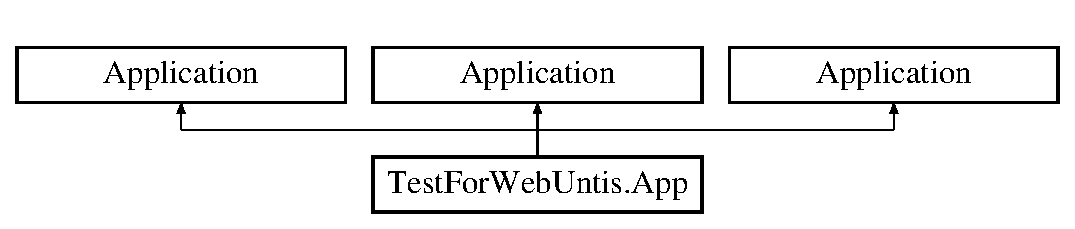
\includegraphics[height=2.000000cm]{class_test_for_web_untis_1_1_app}
\end{center}
\end{figure}
\subsection*{Öffentliche Methoden}
\begin{DoxyCompactItemize}
\item 
\hyperlink{class_test_for_web_untis_1_1_app_a1cfa227a9beb595ed54f345673442556}{App} ()
\begin{DoxyCompactList}\small\item\em Konstruktor für das Application-\/\-Objekt. \end{DoxyCompactList}\item 
void \hyperlink{class_test_for_web_untis_1_1_app_a010a481103b741a79d7b6d3e4bf36efd}{Initialize\-Component} ()
\begin{DoxyCompactList}\small\item\em Initialize\-Component \end{DoxyCompactList}\item 
void \hyperlink{class_test_for_web_untis_1_1_app_a010a481103b741a79d7b6d3e4bf36efd}{Initialize\-Component} ()
\begin{DoxyCompactList}\small\item\em Initialize\-Component \end{DoxyCompactList}\end{DoxyCompactItemize}
\subsection*{Propertys}
\begin{DoxyCompactItemize}
\item 
Phone\-Application\-Frame \hyperlink{class_test_for_web_untis_1_1_app_a3de6c087bb9af076ec1ee6eaf47f5cfa}{Root\-Frame}\hspace{0.3cm}{\ttfamily  \mbox{[}get, set\mbox{]}}
\begin{DoxyCompactList}\small\item\em Bietet einen einfachen Zugriff auf den Stammframe der Phone-\/\-Anwendung. \end{DoxyCompactList}\end{DoxyCompactItemize}


\subsection{Beschreibung der Konstruktoren und Destruktoren}
\hypertarget{class_test_for_web_untis_1_1_app_a1cfa227a9beb595ed54f345673442556}{\index{Test\-For\-Web\-Untis\-::\-App@{Test\-For\-Web\-Untis\-::\-App}!App@{App}}
\index{App@{App}!TestForWebUntis::App@{Test\-For\-Web\-Untis\-::\-App}}
\subsubsection[{App}]{\setlength{\rightskip}{0pt plus 5cm}Test\-For\-Web\-Untis.\-App.\-App (
\begin{DoxyParamCaption}
{}
\end{DoxyParamCaption}
)\hspace{0.3cm}{\ttfamily [inline]}}}\label{class_test_for_web_untis_1_1_app_a1cfa227a9beb595ed54f345673442556}


Konstruktor für das Application-\/\-Objekt. 



\subsection{Dokumentation der Elementfunktionen}
\hypertarget{class_test_for_web_untis_1_1_app_a010a481103b741a79d7b6d3e4bf36efd}{\index{Test\-For\-Web\-Untis\-::\-App@{Test\-For\-Web\-Untis\-::\-App}!Initialize\-Component@{Initialize\-Component}}
\index{Initialize\-Component@{Initialize\-Component}!TestForWebUntis::App@{Test\-For\-Web\-Untis\-::\-App}}
\subsubsection[{Initialize\-Component}]{\setlength{\rightskip}{0pt plus 5cm}void Test\-For\-Web\-Untis.\-App.\-Initialize\-Component (
\begin{DoxyParamCaption}
{}
\end{DoxyParamCaption}
)\hspace{0.3cm}{\ttfamily [inline]}}}\label{class_test_for_web_untis_1_1_app_a010a481103b741a79d7b6d3e4bf36efd}


Initialize\-Component 

\hypertarget{class_test_for_web_untis_1_1_app_a010a481103b741a79d7b6d3e4bf36efd}{\index{Test\-For\-Web\-Untis\-::\-App@{Test\-For\-Web\-Untis\-::\-App}!Initialize\-Component@{Initialize\-Component}}
\index{Initialize\-Component@{Initialize\-Component}!TestForWebUntis::App@{Test\-For\-Web\-Untis\-::\-App}}
\subsubsection[{Initialize\-Component}]{\setlength{\rightskip}{0pt plus 5cm}void Test\-For\-Web\-Untis.\-App.\-Initialize\-Component (
\begin{DoxyParamCaption}
{}
\end{DoxyParamCaption}
)\hspace{0.3cm}{\ttfamily [inline]}}}\label{class_test_for_web_untis_1_1_app_a010a481103b741a79d7b6d3e4bf36efd}


Initialize\-Component 



\subsection{Dokumentation der Propertys}
\hypertarget{class_test_for_web_untis_1_1_app_a3de6c087bb9af076ec1ee6eaf47f5cfa}{\index{Test\-For\-Web\-Untis\-::\-App@{Test\-For\-Web\-Untis\-::\-App}!Root\-Frame@{Root\-Frame}}
\index{Root\-Frame@{Root\-Frame}!TestForWebUntis::App@{Test\-For\-Web\-Untis\-::\-App}}
\subsubsection[{Root\-Frame}]{\setlength{\rightskip}{0pt plus 5cm}Phone\-Application\-Frame Test\-For\-Web\-Untis.\-App.\-Root\-Frame\hspace{0.3cm}{\ttfamily [get]}, {\ttfamily [set]}}}\label{class_test_for_web_untis_1_1_app_a3de6c087bb9af076ec1ee6eaf47f5cfa}


Bietet einen einfachen Zugriff auf den Stammframe der Phone-\/\-Anwendung. 

\begin{DoxyReturn}{Rückgabe}
Der Stammframe der Phone-\/\-Anwendung.
\end{DoxyReturn}


Die Dokumentation für diese Klasse wurde erzeugt aufgrund der Dateien\-:\begin{DoxyCompactItemize}
\item 
C\-:/\-Users/fabian.\-franz/\-Documents/\-Git\-Hub/\-H\-T\-L\-\_\-\-W\-L\-A\-\_\-\-W\-E\-B\-U/\-Code/\-A\-P\-I/\-Test\-For\-Web\-Untis/\-Test\-For\-Web\-Untis/App.\-xaml.\-cs\item 
C\-:/\-Users/fabian.\-franz/\-Documents/\-Git\-Hub/\-H\-T\-L\-\_\-\-W\-L\-A\-\_\-\-W\-E\-B\-U/\-Code/\-A\-P\-I/\-Test\-For\-Web\-Untis/\-Test\-For\-Web\-Untis/obj/\-Debug/App.\-g.\-cs\item 
C\-:/\-Users/fabian.\-franz/\-Documents/\-Git\-Hub/\-H\-T\-L\-\_\-\-W\-L\-A\-\_\-\-W\-E\-B\-U/\-Code/\-A\-P\-I/\-Test\-For\-Web\-Untis/\-Test\-For\-Web\-Untis/obj/\-Debug/App.\-g.\-i.\-cs\end{DoxyCompactItemize}

\hypertarget{struct_webuntis_a_p_i_1_1_types_1_1_department}{\section{Webuntis\-A\-P\-I.\-Types.\-Department Strukturreferenz}
\label{struct_webuntis_a_p_i_1_1_types_1_1_department}\index{Webuntis\-A\-P\-I.\-Types.\-Department@{Webuntis\-A\-P\-I.\-Types.\-Department}}
}


\hyperlink{struct_webuntis_a_p_i_1_1_types_1_1_department}{Webuntis\-A\-P\-I\-::\-Types\-::\-Department}.  


\subsection*{Öffentliche Attribute}
\begin{DoxyCompactItemize}
\item 
int \hyperlink{struct_webuntis_a_p_i_1_1_types_1_1_department_a543d6d34378c9649d7cf72ea88bfbb61}{id}
\item 
String \hyperlink{struct_webuntis_a_p_i_1_1_types_1_1_department_aa2a3990003b54bc6a9946be1c2ab5572}{name}
\item 
String \hyperlink{struct_webuntis_a_p_i_1_1_types_1_1_department_ac9d9a76d977fbdccfd18a7f88c88fbac}{longname}
\end{DoxyCompactItemize}


\subsection{Ausführliche Beschreibung}
\hyperlink{struct_webuntis_a_p_i_1_1_types_1_1_department}{Webuntis\-A\-P\-I\-::\-Types\-::\-Department}. 

The Structure to save information about a \hyperlink{struct_webuntis_a_p_i_1_1_types_1_1_department}{Department} -\/ really not important but A\-P\-I gives it 

\subsection{Dokumentation der Datenelemente}
\hypertarget{struct_webuntis_a_p_i_1_1_types_1_1_department_a543d6d34378c9649d7cf72ea88bfbb61}{\index{Webuntis\-A\-P\-I\-::\-Types\-::\-Department@{Webuntis\-A\-P\-I\-::\-Types\-::\-Department}!id@{id}}
\index{id@{id}!WebuntisAPI::Types::Department@{Webuntis\-A\-P\-I\-::\-Types\-::\-Department}}
\subsubsection[{id}]{\setlength{\rightskip}{0pt plus 5cm}int Webuntis\-A\-P\-I.\-Types.\-Department.\-id}}\label{struct_webuntis_a_p_i_1_1_types_1_1_department_a543d6d34378c9649d7cf72ea88bfbb61}
Field containing id \hypertarget{struct_webuntis_a_p_i_1_1_types_1_1_department_ac9d9a76d977fbdccfd18a7f88c88fbac}{\index{Webuntis\-A\-P\-I\-::\-Types\-::\-Department@{Webuntis\-A\-P\-I\-::\-Types\-::\-Department}!longname@{longname}}
\index{longname@{longname}!WebuntisAPI::Types::Department@{Webuntis\-A\-P\-I\-::\-Types\-::\-Department}}
\subsubsection[{longname}]{\setlength{\rightskip}{0pt plus 5cm}String Webuntis\-A\-P\-I.\-Types.\-Department.\-longname}}\label{struct_webuntis_a_p_i_1_1_types_1_1_department_ac9d9a76d977fbdccfd18a7f88c88fbac}
Field containing long name of department \hypertarget{struct_webuntis_a_p_i_1_1_types_1_1_department_aa2a3990003b54bc6a9946be1c2ab5572}{\index{Webuntis\-A\-P\-I\-::\-Types\-::\-Department@{Webuntis\-A\-P\-I\-::\-Types\-::\-Department}!name@{name}}
\index{name@{name}!WebuntisAPI::Types::Department@{Webuntis\-A\-P\-I\-::\-Types\-::\-Department}}
\subsubsection[{name}]{\setlength{\rightskip}{0pt plus 5cm}String Webuntis\-A\-P\-I.\-Types.\-Department.\-name}}\label{struct_webuntis_a_p_i_1_1_types_1_1_department_aa2a3990003b54bc6a9946be1c2ab5572}
Field containing short name of department 

Die Dokumentation für diese Struktur wurde erzeugt aufgrund der Datei\-:\begin{DoxyCompactItemize}
\item 
C\-:/\-Users/fabian.\-franz/\-Documents/\-Git\-Hub/\-H\-T\-L\-\_\-\-W\-L\-A\-\_\-\-W\-E\-B\-U/\-Code/\-A\-P\-I/\-Test\-For\-Web\-Untis/\-Test\-For\-Web\-Untis/Web\-Untis.\-cs\end{DoxyCompactItemize}

\hypertarget{struct_webuntis_a_p_i_1_1_types_1_1_holiday}{\section{Webuntis\-A\-P\-I.\-Types.\-Holiday Strukturreferenz}
\label{struct_webuntis_a_p_i_1_1_types_1_1_holiday}\index{Webuntis\-A\-P\-I.\-Types.\-Holiday@{Webuntis\-A\-P\-I.\-Types.\-Holiday}}
}


\hyperlink{struct_webuntis_a_p_i_1_1_types_1_1_holiday}{Webuntis\-A\-P\-I\-::\-Types\-::\-Holiday}.  


\subsection*{Öffentliche Attribute}
\begin{DoxyCompactItemize}
\item 
int \hyperlink{struct_webuntis_a_p_i_1_1_types_1_1_holiday_af850132078feaf8f2395e20a0800d74a}{id}
\item 
String \hyperlink{struct_webuntis_a_p_i_1_1_types_1_1_holiday_a092c9f61df2c8287135afb4551cbacdc}{name}
\item 
String \hyperlink{struct_webuntis_a_p_i_1_1_types_1_1_holiday_afb7e41fafeec189033e04da99946817f}{longname}
\item 
Date\-Time \hyperlink{struct_webuntis_a_p_i_1_1_types_1_1_holiday_a489a91e746530bfed3300c39533297f1}{start\-Time}
\item 
Date\-Time \hyperlink{struct_webuntis_a_p_i_1_1_types_1_1_holiday_a8554b4c5a0b600762065145df7666519}{end\-Time}
\end{DoxyCompactItemize}


\subsection{Ausführliche Beschreibung}
\hyperlink{struct_webuntis_a_p_i_1_1_types_1_1_holiday}{Webuntis\-A\-P\-I\-::\-Types\-::\-Holiday}. 

The Structure to save information about a holidays 

\subsection{Dokumentation der Datenelemente}
\hypertarget{struct_webuntis_a_p_i_1_1_types_1_1_holiday_a8554b4c5a0b600762065145df7666519}{\index{Webuntis\-A\-P\-I\-::\-Types\-::\-Holiday@{Webuntis\-A\-P\-I\-::\-Types\-::\-Holiday}!end\-Time@{end\-Time}}
\index{end\-Time@{end\-Time}!WebuntisAPI::Types::Holiday@{Webuntis\-A\-P\-I\-::\-Types\-::\-Holiday}}
\subsubsection[{end\-Time}]{\setlength{\rightskip}{0pt plus 5cm}Date\-Time Webuntis\-A\-P\-I.\-Types.\-Holiday.\-end\-Time}}\label{struct_webuntis_a_p_i_1_1_types_1_1_holiday_a8554b4c5a0b600762065145df7666519}
Field containing endtime of holiday \hypertarget{struct_webuntis_a_p_i_1_1_types_1_1_holiday_af850132078feaf8f2395e20a0800d74a}{\index{Webuntis\-A\-P\-I\-::\-Types\-::\-Holiday@{Webuntis\-A\-P\-I\-::\-Types\-::\-Holiday}!id@{id}}
\index{id@{id}!WebuntisAPI::Types::Holiday@{Webuntis\-A\-P\-I\-::\-Types\-::\-Holiday}}
\subsubsection[{id}]{\setlength{\rightskip}{0pt plus 5cm}int Webuntis\-A\-P\-I.\-Types.\-Holiday.\-id}}\label{struct_webuntis_a_p_i_1_1_types_1_1_holiday_af850132078feaf8f2395e20a0800d74a}
Field containing id \hypertarget{struct_webuntis_a_p_i_1_1_types_1_1_holiday_afb7e41fafeec189033e04da99946817f}{\index{Webuntis\-A\-P\-I\-::\-Types\-::\-Holiday@{Webuntis\-A\-P\-I\-::\-Types\-::\-Holiday}!longname@{longname}}
\index{longname@{longname}!WebuntisAPI::Types::Holiday@{Webuntis\-A\-P\-I\-::\-Types\-::\-Holiday}}
\subsubsection[{longname}]{\setlength{\rightskip}{0pt plus 5cm}String Webuntis\-A\-P\-I.\-Types.\-Holiday.\-longname}}\label{struct_webuntis_a_p_i_1_1_types_1_1_holiday_afb7e41fafeec189033e04da99946817f}
Field containing long name of holiday \hypertarget{struct_webuntis_a_p_i_1_1_types_1_1_holiday_a092c9f61df2c8287135afb4551cbacdc}{\index{Webuntis\-A\-P\-I\-::\-Types\-::\-Holiday@{Webuntis\-A\-P\-I\-::\-Types\-::\-Holiday}!name@{name}}
\index{name@{name}!WebuntisAPI::Types::Holiday@{Webuntis\-A\-P\-I\-::\-Types\-::\-Holiday}}
\subsubsection[{name}]{\setlength{\rightskip}{0pt plus 5cm}String Webuntis\-A\-P\-I.\-Types.\-Holiday.\-name}}\label{struct_webuntis_a_p_i_1_1_types_1_1_holiday_a092c9f61df2c8287135afb4551cbacdc}
Field containing name of holiday \hypertarget{struct_webuntis_a_p_i_1_1_types_1_1_holiday_a489a91e746530bfed3300c39533297f1}{\index{Webuntis\-A\-P\-I\-::\-Types\-::\-Holiday@{Webuntis\-A\-P\-I\-::\-Types\-::\-Holiday}!start\-Time@{start\-Time}}
\index{start\-Time@{start\-Time}!WebuntisAPI::Types::Holiday@{Webuntis\-A\-P\-I\-::\-Types\-::\-Holiday}}
\subsubsection[{start\-Time}]{\setlength{\rightskip}{0pt plus 5cm}Date\-Time Webuntis\-A\-P\-I.\-Types.\-Holiday.\-start\-Time}}\label{struct_webuntis_a_p_i_1_1_types_1_1_holiday_a489a91e746530bfed3300c39533297f1}
Field containing starttime of holiday 

Die Dokumentation für diese Struktur wurde erzeugt aufgrund der Datei\-:\begin{DoxyCompactItemize}
\item 
C\-:/\-Users/fabian.\-franz/\-Documents/\-Git\-Hub/\-H\-T\-L\-\_\-\-W\-L\-A\-\_\-\-W\-E\-B\-U/\-Code/\-A\-P\-I/\-Test\-For\-Web\-Untis/\-Test\-For\-Web\-Untis/Web\-Untis.\-cs\end{DoxyCompactItemize}

\hypertarget{class_download_1_1_http_web_request___begin_get_response}{\section{Download.\-Http\-Web\-Request\-\_\-\-Begin\-Get\-Response Klassenreferenz}
\label{class_download_1_1_http_web_request___begin_get_response}\index{Download.\-Http\-Web\-Request\-\_\-\-Begin\-Get\-Response@{Download.\-Http\-Web\-Request\-\_\-\-Begin\-Get\-Response}}
}
\subsection*{Statische öffentliche Attribute}
\begin{DoxyCompactItemize}
\item 
static Manual\-Reset\-Event \hyperlink{class_download_1_1_http_web_request___begin_get_response_abf8ceb91508e305aa886e05eaed3737e}{all\-Done} = new Manual\-Reset\-Event(false)
\end{DoxyCompactItemize}


\subsection{Dokumentation der Datenelemente}
\hypertarget{class_download_1_1_http_web_request___begin_get_response_abf8ceb91508e305aa886e05eaed3737e}{\index{Download\-::\-Http\-Web\-Request\-\_\-\-Begin\-Get\-Response@{Download\-::\-Http\-Web\-Request\-\_\-\-Begin\-Get\-Response}!all\-Done@{all\-Done}}
\index{all\-Done@{all\-Done}!Download::HttpWebRequest_BeginGetResponse@{Download\-::\-Http\-Web\-Request\-\_\-\-Begin\-Get\-Response}}
\subsubsection[{all\-Done}]{\setlength{\rightskip}{0pt plus 5cm}Manual\-Reset\-Event Download.\-Http\-Web\-Request\-\_\-\-Begin\-Get\-Response.\-all\-Done = new Manual\-Reset\-Event(false)\hspace{0.3cm}{\ttfamily [static]}}}\label{class_download_1_1_http_web_request___begin_get_response_abf8ceb91508e305aa886e05eaed3737e}
Information if done 

Die Dokumentation für diese Klasse wurde erzeugt aufgrund der Datei\-:\begin{DoxyCompactItemize}
\item 
C\-:/\-Users/fabian.\-franz/\-Documents/\-Git\-Hub/\-H\-T\-L\-\_\-\-W\-L\-A\-\_\-\-W\-E\-B\-U/\-Code/\-A\-P\-I/\-Test\-For\-Web\-Untis/\-Test\-For\-Web\-Untis/Web\-Untis.\-cs\end{DoxyCompactItemize}

\hypertarget{class_do_download_1_1_http_web_request___begin_get_response}{\section{Do\-Download.\-Http\-Web\-Request\-\_\-\-Begin\-Get\-Response Klassenreferenz}
\label{class_do_download_1_1_http_web_request___begin_get_response}\index{Do\-Download.\-Http\-Web\-Request\-\_\-\-Begin\-Get\-Response@{Do\-Download.\-Http\-Web\-Request\-\_\-\-Begin\-Get\-Response}}
}


\hyperlink{class_do_download_1_1_http_web_request___begin_get_response}{Do\-Download\-::\-Http\-Web\-Request\-\_\-\-Begin\-Get\-Response}.  


\subsection*{Öffentliche Methoden}
\begin{DoxyCompactItemize}
\item 
void \hyperlink{class_do_download_1_1_http_web_request___begin_get_response_a606b2dabbf563182262cb028cd32c62b}{start} ()
\begin{DoxyCompactList}\small\item\em \hyperlink{class_do_download_1_1_http_web_request___begin_get_response_a606b2dabbf563182262cb028cd32c62b}{start()} \end{DoxyCompactList}\end{DoxyCompactItemize}
\subsection*{Statische öffentliche Attribute}
\begin{DoxyCompactItemize}
\item 
static Manual\-Reset\-Event \hyperlink{class_do_download_1_1_http_web_request___begin_get_response_a03670e4a51868848ede5ca7c7382066a}{all\-Done} = new Manual\-Reset\-Event(false)
\end{DoxyCompactItemize}


\subsection{Ausführliche Beschreibung}
\hyperlink{class_do_download_1_1_http_web_request___begin_get_response}{Do\-Download\-::\-Http\-Web\-Request\-\_\-\-Begin\-Get\-Response}. 

Class to load 

\subsection{Dokumentation der Elementfunktionen}
\hypertarget{class_do_download_1_1_http_web_request___begin_get_response_a606b2dabbf563182262cb028cd32c62b}{\index{Do\-Download\-::\-Http\-Web\-Request\-\_\-\-Begin\-Get\-Response@{Do\-Download\-::\-Http\-Web\-Request\-\_\-\-Begin\-Get\-Response}!start@{start}}
\index{start@{start}!DoDownload::HttpWebRequest_BeginGetResponse@{Do\-Download\-::\-Http\-Web\-Request\-\_\-\-Begin\-Get\-Response}}
\subsubsection[{start}]{\setlength{\rightskip}{0pt plus 5cm}void Do\-Download.\-Http\-Web\-Request\-\_\-\-Begin\-Get\-Response.\-start (
\begin{DoxyParamCaption}
{}
\end{DoxyParamCaption}
)\hspace{0.3cm}{\ttfamily [inline]}}}\label{class_do_download_1_1_http_web_request___begin_get_response_a606b2dabbf563182262cb028cd32c62b}


\hyperlink{class_do_download_1_1_http_web_request___begin_get_response_a606b2dabbf563182262cb028cd32c62b}{start()} 

Starts a Webrequest set the Http\-Web\-Request variables

\begin{DoxyVerb}              If you are behind a firewall and you do not have your browser proxy setup
              you need to use the following proxy creation code.
\end{DoxyVerb}


Create a proxy object. Web\-Proxy my\-Proxy = new Web\-Proxy();

Associate a new Uri object to the \-\_\-w\-Proxy object, using the proxy address selected by the user. my\-Proxy.\-Address = new Uri(\char`\"{}http\-://myproxy\char`\"{});

Finally, initialize the Web request object proxy property with the \-\_\-w\-Proxy object. my\-Http\-Web\-Request.\-Proxy=my\-Proxy;

\subsection{Dokumentation der Datenelemente}
\hypertarget{class_do_download_1_1_http_web_request___begin_get_response_a03670e4a51868848ede5ca7c7382066a}{\index{Do\-Download\-::\-Http\-Web\-Request\-\_\-\-Begin\-Get\-Response@{Do\-Download\-::\-Http\-Web\-Request\-\_\-\-Begin\-Get\-Response}!all\-Done@{all\-Done}}
\index{all\-Done@{all\-Done}!DoDownload::HttpWebRequest_BeginGetResponse@{Do\-Download\-::\-Http\-Web\-Request\-\_\-\-Begin\-Get\-Response}}
\subsubsection[{all\-Done}]{\setlength{\rightskip}{0pt plus 5cm}Manual\-Reset\-Event Do\-Download.\-Http\-Web\-Request\-\_\-\-Begin\-Get\-Response.\-all\-Done = new Manual\-Reset\-Event(false)\hspace{0.3cm}{\ttfamily [static]}}}\label{class_do_download_1_1_http_web_request___begin_get_response_a03670e4a51868848ede5ca7c7382066a}
Contains the State of the \hyperlink{namespace_download}{Download} 

Die Dokumentation für diese Klasse wurde erzeugt aufgrund der Datei\-:\begin{DoxyCompactItemize}
\item 
C\-:/\-Users/fabian.\-franz/\-Documents/\-Git\-Hub/\-H\-T\-L\-\_\-\-W\-L\-A\-\_\-\-W\-E\-B\-U/\-Code/\-A\-P\-I/\-Test\-For\-Web\-Untis/\-Test\-For\-Web\-Untis/Web\-Untis.\-cs\end{DoxyCompactItemize}

\hypertarget{struct_webuntis_a_p_i_1_1_types_1_1_klasse}{\section{Webuntis\-A\-P\-I.\-Types.\-Klasse Strukturreferenz}
\label{struct_webuntis_a_p_i_1_1_types_1_1_klasse}\index{Webuntis\-A\-P\-I.\-Types.\-Klasse@{Webuntis\-A\-P\-I.\-Types.\-Klasse}}
}


\hyperlink{struct_webuntis_a_p_i_1_1_types_1_1_klasse}{Webuntis\-A\-P\-I\-::\-Types\-::\-Klasse}.  


\subsection*{Öffentliche Attribute}
\begin{DoxyCompactItemize}
\item 
int \hyperlink{struct_webuntis_a_p_i_1_1_types_1_1_klasse_a0c8d6c1ce71142b67d20df2c818bbc75}{id}
\item 
String \hyperlink{struct_webuntis_a_p_i_1_1_types_1_1_klasse_a034b759d9d7262da6eaa0613d5f6a0e7}{name}
\item 
String \hyperlink{struct_webuntis_a_p_i_1_1_types_1_1_klasse_a0ec00ea38031e97b255fa139387142e7}{longname}
\item 
\hypertarget{struct_webuntis_a_p_i_1_1_types_1_1_klasse_a0441c438c8e4098068dadb84615d847e}{int {\bfseries did}}\label{struct_webuntis_a_p_i_1_1_types_1_1_klasse_a0441c438c8e4098068dadb84615d847e}

\end{DoxyCompactItemize}


\subsection{Ausführliche Beschreibung}
\hyperlink{struct_webuntis_a_p_i_1_1_types_1_1_klasse}{Webuntis\-A\-P\-I\-::\-Types\-::\-Klasse}. 

The Structure to save information about a Schoolclass in german because class makes problems 

\subsection{Dokumentation der Datenelemente}
\hypertarget{struct_webuntis_a_p_i_1_1_types_1_1_klasse_a0c8d6c1ce71142b67d20df2c818bbc75}{\index{Webuntis\-A\-P\-I\-::\-Types\-::\-Klasse@{Webuntis\-A\-P\-I\-::\-Types\-::\-Klasse}!id@{id}}
\index{id@{id}!WebuntisAPI::Types::Klasse@{Webuntis\-A\-P\-I\-::\-Types\-::\-Klasse}}
\subsubsection[{id}]{\setlength{\rightskip}{0pt plus 5cm}int Webuntis\-A\-P\-I.\-Types.\-Klasse.\-id}}\label{struct_webuntis_a_p_i_1_1_types_1_1_klasse_a0c8d6c1ce71142b67d20df2c818bbc75}
Field containing id \hypertarget{struct_webuntis_a_p_i_1_1_types_1_1_klasse_a0ec00ea38031e97b255fa139387142e7}{\index{Webuntis\-A\-P\-I\-::\-Types\-::\-Klasse@{Webuntis\-A\-P\-I\-::\-Types\-::\-Klasse}!longname@{longname}}
\index{longname@{longname}!WebuntisAPI::Types::Klasse@{Webuntis\-A\-P\-I\-::\-Types\-::\-Klasse}}
\subsubsection[{longname}]{\setlength{\rightskip}{0pt plus 5cm}String Webuntis\-A\-P\-I.\-Types.\-Klasse.\-longname}}\label{struct_webuntis_a_p_i_1_1_types_1_1_klasse_a0ec00ea38031e97b255fa139387142e7}
Field containing classname \hypertarget{struct_webuntis_a_p_i_1_1_types_1_1_klasse_a034b759d9d7262da6eaa0613d5f6a0e7}{\index{Webuntis\-A\-P\-I\-::\-Types\-::\-Klasse@{Webuntis\-A\-P\-I\-::\-Types\-::\-Klasse}!name@{name}}
\index{name@{name}!WebuntisAPI::Types::Klasse@{Webuntis\-A\-P\-I\-::\-Types\-::\-Klasse}}
\subsubsection[{name}]{\setlength{\rightskip}{0pt plus 5cm}String Webuntis\-A\-P\-I.\-Types.\-Klasse.\-name}}\label{struct_webuntis_a_p_i_1_1_types_1_1_klasse_a034b759d9d7262da6eaa0613d5f6a0e7}
Field containing short classname 

Die Dokumentation für diese Struktur wurde erzeugt aufgrund der Datei\-:\begin{DoxyCompactItemize}
\item 
C\-:/\-Users/fabian.\-franz/\-Documents/\-Git\-Hub/\-H\-T\-L\-\_\-\-W\-L\-A\-\_\-\-W\-E\-B\-U/\-Code/\-A\-P\-I/\-Test\-For\-Web\-Untis/\-Test\-For\-Web\-Untis/Web\-Untis.\-cs\end{DoxyCompactItemize}

\hypertarget{class_test_for_web_untis_1_1_main_page}{\section{Test\-For\-Web\-Untis.\-Main\-Page Klassenreferenz}
\label{class_test_for_web_untis_1_1_main_page}\index{Test\-For\-Web\-Untis.\-Main\-Page@{Test\-For\-Web\-Untis.\-Main\-Page}}
}
Klassendiagramm für Test\-For\-Web\-Untis.\-Main\-Page\-:\begin{figure}[H]
\begin{center}
\leavevmode
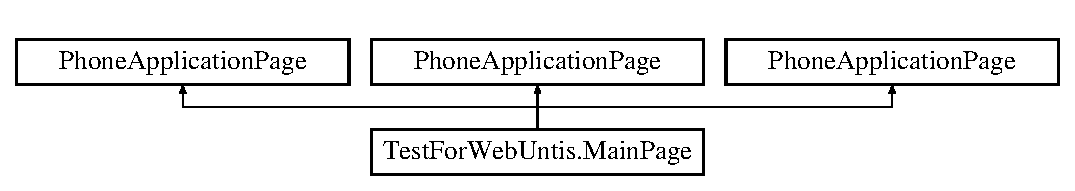
\includegraphics[height=2.000000cm]{class_test_for_web_untis_1_1_main_page}
\end{center}
\end{figure}
\subsection*{Öffentliche Methoden}
\begin{DoxyCompactItemize}
\item 
void \hyperlink{class_test_for_web_untis_1_1_main_page_ab6a5d1396d93a1c7b7bd030b1d406358}{Initialize\-Component} ()
\begin{DoxyCompactList}\small\item\em Initialize\-Component \end{DoxyCompactList}\item 
void \hyperlink{class_test_for_web_untis_1_1_main_page_ab6a5d1396d93a1c7b7bd030b1d406358}{Initialize\-Component} ()
\begin{DoxyCompactList}\small\item\em Initialize\-Component \end{DoxyCompactList}\end{DoxyCompactItemize}


\subsection{Dokumentation der Elementfunktionen}
\hypertarget{class_test_for_web_untis_1_1_main_page_ab6a5d1396d93a1c7b7bd030b1d406358}{\index{Test\-For\-Web\-Untis\-::\-Main\-Page@{Test\-For\-Web\-Untis\-::\-Main\-Page}!Initialize\-Component@{Initialize\-Component}}
\index{Initialize\-Component@{Initialize\-Component}!TestForWebUntis::MainPage@{Test\-For\-Web\-Untis\-::\-Main\-Page}}
\subsubsection[{Initialize\-Component}]{\setlength{\rightskip}{0pt plus 5cm}void Test\-For\-Web\-Untis.\-Main\-Page.\-Initialize\-Component (
\begin{DoxyParamCaption}
{}
\end{DoxyParamCaption}
)\hspace{0.3cm}{\ttfamily [inline]}}}\label{class_test_for_web_untis_1_1_main_page_ab6a5d1396d93a1c7b7bd030b1d406358}


Initialize\-Component 

\hypertarget{class_test_for_web_untis_1_1_main_page_ab6a5d1396d93a1c7b7bd030b1d406358}{\index{Test\-For\-Web\-Untis\-::\-Main\-Page@{Test\-For\-Web\-Untis\-::\-Main\-Page}!Initialize\-Component@{Initialize\-Component}}
\index{Initialize\-Component@{Initialize\-Component}!TestForWebUntis::MainPage@{Test\-For\-Web\-Untis\-::\-Main\-Page}}
\subsubsection[{Initialize\-Component}]{\setlength{\rightskip}{0pt plus 5cm}void Test\-For\-Web\-Untis.\-Main\-Page.\-Initialize\-Component (
\begin{DoxyParamCaption}
{}
\end{DoxyParamCaption}
)\hspace{0.3cm}{\ttfamily [inline]}}}\label{class_test_for_web_untis_1_1_main_page_ab6a5d1396d93a1c7b7bd030b1d406358}


Initialize\-Component 



Die Dokumentation für diese Klasse wurde erzeugt aufgrund der Dateien\-:\begin{DoxyCompactItemize}
\item 
C\-:/\-Users/fabian.\-franz/\-Documents/\-Git\-Hub/\-H\-T\-L\-\_\-\-W\-L\-A\-\_\-\-W\-E\-B\-U/\-Code/\-A\-P\-I/\-Test\-For\-Web\-Untis/\-Test\-For\-Web\-Untis/Main\-Page.\-xaml.\-cs\item 
C\-:/\-Users/fabian.\-franz/\-Documents/\-Git\-Hub/\-H\-T\-L\-\_\-\-W\-L\-A\-\_\-\-W\-E\-B\-U/\-Code/\-A\-P\-I/\-Test\-For\-Web\-Untis/\-Test\-For\-Web\-Untis/obj/\-Debug/Main\-Page.\-g.\-cs\item 
C\-:/\-Users/fabian.\-franz/\-Documents/\-Git\-Hub/\-H\-T\-L\-\_\-\-W\-L\-A\-\_\-\-W\-E\-B\-U/\-Code/\-A\-P\-I/\-Test\-For\-Web\-Untis/\-Test\-For\-Web\-Untis/obj/\-Debug/Main\-Page.\-g.\-i.\-cs\end{DoxyCompactItemize}

\hypertarget{class_do_download_1_1_request_state}{\section{Do\-Download.\-Request\-State Klassenreferenz}
\label{class_do_download_1_1_request_state}\index{Do\-Download.\-Request\-State@{Do\-Download.\-Request\-State}}
}


\hyperlink{class_do_download_1_1_request_state}{Do\-Download\-::\-Request\-State}.  


\subsection*{Öffentliche Attribute}
\begin{DoxyCompactItemize}
\item 
String\-Builder \hyperlink{class_do_download_1_1_request_state_af0c123367214a73fda316c1e53f35c9b}{request\-Data}
\item 
byte\mbox{[}$\,$\mbox{]} \hyperlink{class_do_download_1_1_request_state_aca28c955c588bc3d14b930bd281a7eb8}{Buffer\-Read}
\item 
Http\-Web\-Request \hyperlink{class_do_download_1_1_request_state_a407f724ed70036cffecc6d595e70b3eb}{request}
\item 
Http\-Web\-Response \hyperlink{class_do_download_1_1_request_state_a92511d66202e453392c09341c2f5a3c6}{response}
\item 
Stream \hyperlink{class_do_download_1_1_request_state_acd2b043e223ba326627ebdc03eba740b}{stream\-Response}
\end{DoxyCompactItemize}


\subsection{Ausführliche Beschreibung}
\hyperlink{class_do_download_1_1_request_state}{Do\-Download\-::\-Request\-State}. 

State of the \hyperlink{namespace_download}{Download} 

\subsection{Dokumentation der Datenelemente}
\hypertarget{class_do_download_1_1_request_state_aca28c955c588bc3d14b930bd281a7eb8}{\index{Do\-Download\-::\-Request\-State@{Do\-Download\-::\-Request\-State}!Buffer\-Read@{Buffer\-Read}}
\index{Buffer\-Read@{Buffer\-Read}!DoDownload::RequestState@{Do\-Download\-::\-Request\-State}}
\subsubsection[{Buffer\-Read}]{\setlength{\rightskip}{0pt plus 5cm}byte \mbox{[}$\,$\mbox{]} Do\-Download.\-Request\-State.\-Buffer\-Read}}\label{class_do_download_1_1_request_state_aca28c955c588bc3d14b930bd281a7eb8}
Buffer to \hyperlink{namespace_download}{Download} the Project \hypertarget{class_do_download_1_1_request_state_a407f724ed70036cffecc6d595e70b3eb}{\index{Do\-Download\-::\-Request\-State@{Do\-Download\-::\-Request\-State}!request@{request}}
\index{request@{request}!DoDownload::RequestState@{Do\-Download\-::\-Request\-State}}
\subsubsection[{request}]{\setlength{\rightskip}{0pt plus 5cm}Http\-Web\-Request Do\-Download.\-Request\-State.\-request}}\label{class_do_download_1_1_request_state_a407f724ed70036cffecc6d595e70b3eb}
The Data to send to the Server \hypertarget{class_do_download_1_1_request_state_af0c123367214a73fda316c1e53f35c9b}{\index{Do\-Download\-::\-Request\-State@{Do\-Download\-::\-Request\-State}!request\-Data@{request\-Data}}
\index{request\-Data@{request\-Data}!DoDownload::RequestState@{Do\-Download\-::\-Request\-State}}
\subsubsection[{request\-Data}]{\setlength{\rightskip}{0pt plus 5cm}String\-Builder Do\-Download.\-Request\-State.\-request\-Data}}\label{class_do_download_1_1_request_state_af0c123367214a73fda316c1e53f35c9b}
An Object to crate a String \hypertarget{class_do_download_1_1_request_state_a92511d66202e453392c09341c2f5a3c6}{\index{Do\-Download\-::\-Request\-State@{Do\-Download\-::\-Request\-State}!response@{response}}
\index{response@{response}!DoDownload::RequestState@{Do\-Download\-::\-Request\-State}}
\subsubsection[{response}]{\setlength{\rightskip}{0pt plus 5cm}Http\-Web\-Response Do\-Download.\-Request\-State.\-response}}\label{class_do_download_1_1_request_state_a92511d66202e453392c09341c2f5a3c6}
The Data to get from the Server \hypertarget{class_do_download_1_1_request_state_acd2b043e223ba326627ebdc03eba740b}{\index{Do\-Download\-::\-Request\-State@{Do\-Download\-::\-Request\-State}!stream\-Response@{stream\-Response}}
\index{stream\-Response@{stream\-Response}!DoDownload::RequestState@{Do\-Download\-::\-Request\-State}}
\subsubsection[{stream\-Response}]{\setlength{\rightskip}{0pt plus 5cm}Stream Do\-Download.\-Request\-State.\-stream\-Response}}\label{class_do_download_1_1_request_state_acd2b043e223ba326627ebdc03eba740b}
The Stream of the Data in the Server 

Die Dokumentation für diese Klasse wurde erzeugt aufgrund der Datei\-:\begin{DoxyCompactItemize}
\item 
C\-:/\-Users/fabian.\-franz/\-Documents/\-Git\-Hub/\-H\-T\-L\-\_\-\-W\-L\-A\-\_\-\-W\-E\-B\-U/\-Code/\-A\-P\-I/\-Test\-For\-Web\-Untis/\-Test\-For\-Web\-Untis/Web\-Untis.\-cs\end{DoxyCompactItemize}

\hypertarget{class_download_1_1_request_state}{\section{Download.\-Request\-State Klassenreferenz}
\label{class_download_1_1_request_state}\index{Download.\-Request\-State@{Download.\-Request\-State}}
}


\hyperlink{class_download_1_1_request_state}{Download\-::\-Request\-State}.  


\subsection*{Öffentliche Methoden}
\begin{DoxyCompactItemize}
\item 
\hypertarget{class_download_1_1_request_state_aecc11124306e2d34e3d7d139571098f6}{\hyperlink{class_download_1_1_request_state_aecc11124306e2d34e3d7d139571098f6}{Request\-State} ()}\label{class_download_1_1_request_state_aecc11124306e2d34e3d7d139571098f6}

\begin{DoxyCompactList}\small\item\em Initialisise Object. \end{DoxyCompactList}\end{DoxyCompactItemize}
\subsection*{Öffentliche Attribute}
\begin{DoxyCompactItemize}
\item 
String\-Builder \hyperlink{class_download_1_1_request_state_ab20c7c09c5efb2e831d8157ac2fea1ae}{request\-Data}
\item 
byte\mbox{[}$\,$\mbox{]} \hyperlink{class_download_1_1_request_state_aec613e05d7ced342aa5d6fb28aff5bc7}{Buffer\-Read}
\item 
Http\-Web\-Request \hyperlink{class_download_1_1_request_state_a0a74186a43e3ed603eb2236b08ecd753}{request}
\item 
Http\-Web\-Response \hyperlink{class_download_1_1_request_state_af85537a87aa3c35d8cc1058e143f4201}{response}
\item 
Stream \hyperlink{class_download_1_1_request_state_a30cef36e2cceb6a4e1b2a446247e60be}{stream\-Response}
\end{DoxyCompactItemize}


\subsection{Ausführliche Beschreibung}
\hyperlink{class_download_1_1_request_state}{Download\-::\-Request\-State}. 

Holds The State of the Dowload 

\subsection{Dokumentation der Datenelemente}
\hypertarget{class_download_1_1_request_state_aec613e05d7ced342aa5d6fb28aff5bc7}{\index{Download\-::\-Request\-State@{Download\-::\-Request\-State}!Buffer\-Read@{Buffer\-Read}}
\index{Buffer\-Read@{Buffer\-Read}!Download::RequestState@{Download\-::\-Request\-State}}
\subsubsection[{Buffer\-Read}]{\setlength{\rightskip}{0pt plus 5cm}byte \mbox{[}$\,$\mbox{]} Download.\-Request\-State.\-Buffer\-Read}}\label{class_download_1_1_request_state_aec613e05d7ced342aa5d6fb28aff5bc7}
This is the \hyperlink{namespace_download}{Download} Buffer itself \hypertarget{class_download_1_1_request_state_a0a74186a43e3ed603eb2236b08ecd753}{\index{Download\-::\-Request\-State@{Download\-::\-Request\-State}!request@{request}}
\index{request@{request}!Download::RequestState@{Download\-::\-Request\-State}}
\subsubsection[{request}]{\setlength{\rightskip}{0pt plus 5cm}Http\-Web\-Request Download.\-Request\-State.\-request}}\label{class_download_1_1_request_state_a0a74186a43e3ed603eb2236b08ecd753}
Object for the Request \hypertarget{class_download_1_1_request_state_ab20c7c09c5efb2e831d8157ac2fea1ae}{\index{Download\-::\-Request\-State@{Download\-::\-Request\-State}!request\-Data@{request\-Data}}
\index{request\-Data@{request\-Data}!Download::RequestState@{Download\-::\-Request\-State}}
\subsubsection[{request\-Data}]{\setlength{\rightskip}{0pt plus 5cm}String\-Builder Download.\-Request\-State.\-request\-Data}}\label{class_download_1_1_request_state_ab20c7c09c5efb2e831d8157ac2fea1ae}
Builds a String like java string builder class \hypertarget{class_download_1_1_request_state_af85537a87aa3c35d8cc1058e143f4201}{\index{Download\-::\-Request\-State@{Download\-::\-Request\-State}!response@{response}}
\index{response@{response}!Download::RequestState@{Download\-::\-Request\-State}}
\subsubsection[{response}]{\setlength{\rightskip}{0pt plus 5cm}Http\-Web\-Response Download.\-Request\-State.\-response}}\label{class_download_1_1_request_state_af85537a87aa3c35d8cc1058e143f4201}
Here is the Answer \hypertarget{class_download_1_1_request_state_a30cef36e2cceb6a4e1b2a446247e60be}{\index{Download\-::\-Request\-State@{Download\-::\-Request\-State}!stream\-Response@{stream\-Response}}
\index{stream\-Response@{stream\-Response}!Download::RequestState@{Download\-::\-Request\-State}}
\subsubsection[{stream\-Response}]{\setlength{\rightskip}{0pt plus 5cm}Stream Download.\-Request\-State.\-stream\-Response}}\label{class_download_1_1_request_state_a30cef36e2cceb6a4e1b2a446247e60be}
Response Stream 

Die Dokumentation für diese Klasse wurde erzeugt aufgrund der Datei\-:\begin{DoxyCompactItemize}
\item 
C\-:/\-Users/fabian.\-franz/\-Documents/\-Git\-Hub/\-H\-T\-L\-\_\-\-W\-L\-A\-\_\-\-W\-E\-B\-U/\-Code/\-A\-P\-I/\-Test\-For\-Web\-Untis/\-Test\-For\-Web\-Untis/Web\-Untis.\-cs\end{DoxyCompactItemize}

\hypertarget{struct_webuntis_a_p_i_1_1_types_1_1_schoolyear}{\section{Webuntis\-A\-P\-I.\-Types.\-Schoolyear Strukturreferenz}
\label{struct_webuntis_a_p_i_1_1_types_1_1_schoolyear}\index{Webuntis\-A\-P\-I.\-Types.\-Schoolyear@{Webuntis\-A\-P\-I.\-Types.\-Schoolyear}}
}


\hyperlink{struct_webuntis_a_p_i_1_1_types_1_1_schoolyear}{Webuntis\-A\-P\-I\-::\-Types\-::\-Schoolyear}.  


\subsection*{Öffentliche Attribute}
\begin{DoxyCompactItemize}
\item 
int \hyperlink{struct_webuntis_a_p_i_1_1_types_1_1_schoolyear_a5919885c6ffc12918b27fb9f13fd2c79}{id}
\item 
String \hyperlink{struct_webuntis_a_p_i_1_1_types_1_1_schoolyear_a230844174db7f59e6536a2083ade0c41}{name}
\item 
Date\-Time \hyperlink{struct_webuntis_a_p_i_1_1_types_1_1_schoolyear_a137e91a773888c2c55dcbe153290e783}{start\-Time}
\item 
Date\-Time \hyperlink{struct_webuntis_a_p_i_1_1_types_1_1_schoolyear_ab90946531bc36b904e2a71b3ee44b03f}{end\-Time}
\end{DoxyCompactItemize}


\subsection{Ausführliche Beschreibung}
\hyperlink{struct_webuntis_a_p_i_1_1_types_1_1_schoolyear}{Webuntis\-A\-P\-I\-::\-Types\-::\-Schoolyear}. 

The Structure to save information about a schoolyear, but I think this is N\-O\-T important 

\subsection{Dokumentation der Datenelemente}
\hypertarget{struct_webuntis_a_p_i_1_1_types_1_1_schoolyear_ab90946531bc36b904e2a71b3ee44b03f}{\index{Webuntis\-A\-P\-I\-::\-Types\-::\-Schoolyear@{Webuntis\-A\-P\-I\-::\-Types\-::\-Schoolyear}!end\-Time@{end\-Time}}
\index{end\-Time@{end\-Time}!WebuntisAPI::Types::Schoolyear@{Webuntis\-A\-P\-I\-::\-Types\-::\-Schoolyear}}
\subsubsection[{end\-Time}]{\setlength{\rightskip}{0pt plus 5cm}Date\-Time Webuntis\-A\-P\-I.\-Types.\-Schoolyear.\-end\-Time}}\label{struct_webuntis_a_p_i_1_1_types_1_1_schoolyear_ab90946531bc36b904e2a71b3ee44b03f}
Field containing last day of shoolyear \hypertarget{struct_webuntis_a_p_i_1_1_types_1_1_schoolyear_a5919885c6ffc12918b27fb9f13fd2c79}{\index{Webuntis\-A\-P\-I\-::\-Types\-::\-Schoolyear@{Webuntis\-A\-P\-I\-::\-Types\-::\-Schoolyear}!id@{id}}
\index{id@{id}!WebuntisAPI::Types::Schoolyear@{Webuntis\-A\-P\-I\-::\-Types\-::\-Schoolyear}}
\subsubsection[{id}]{\setlength{\rightskip}{0pt plus 5cm}int Webuntis\-A\-P\-I.\-Types.\-Schoolyear.\-id}}\label{struct_webuntis_a_p_i_1_1_types_1_1_schoolyear_a5919885c6ffc12918b27fb9f13fd2c79}
Field containing id \hypertarget{struct_webuntis_a_p_i_1_1_types_1_1_schoolyear_a230844174db7f59e6536a2083ade0c41}{\index{Webuntis\-A\-P\-I\-::\-Types\-::\-Schoolyear@{Webuntis\-A\-P\-I\-::\-Types\-::\-Schoolyear}!name@{name}}
\index{name@{name}!WebuntisAPI::Types::Schoolyear@{Webuntis\-A\-P\-I\-::\-Types\-::\-Schoolyear}}
\subsubsection[{name}]{\setlength{\rightskip}{0pt plus 5cm}String Webuntis\-A\-P\-I.\-Types.\-Schoolyear.\-name}}\label{struct_webuntis_a_p_i_1_1_types_1_1_schoolyear_a230844174db7f59e6536a2083ade0c41}
Field containing name of shoolyear \hypertarget{struct_webuntis_a_p_i_1_1_types_1_1_schoolyear_a137e91a773888c2c55dcbe153290e783}{\index{Webuntis\-A\-P\-I\-::\-Types\-::\-Schoolyear@{Webuntis\-A\-P\-I\-::\-Types\-::\-Schoolyear}!start\-Time@{start\-Time}}
\index{start\-Time@{start\-Time}!WebuntisAPI::Types::Schoolyear@{Webuntis\-A\-P\-I\-::\-Types\-::\-Schoolyear}}
\subsubsection[{start\-Time}]{\setlength{\rightskip}{0pt plus 5cm}Date\-Time Webuntis\-A\-P\-I.\-Types.\-Schoolyear.\-start\-Time}}\label{struct_webuntis_a_p_i_1_1_types_1_1_schoolyear_a137e91a773888c2c55dcbe153290e783}
Field containing first day of schoolyear 

Die Dokumentation für diese Struktur wurde erzeugt aufgrund der Datei\-:\begin{DoxyCompactItemize}
\item 
C\-:/\-Users/fabian.\-franz/\-Documents/\-Git\-Hub/\-H\-T\-L\-\_\-\-W\-L\-A\-\_\-\-W\-E\-B\-U/\-Code/\-A\-P\-I/\-Test\-For\-Web\-Untis/\-Test\-For\-Web\-Untis/Web\-Untis.\-cs\end{DoxyCompactItemize}

\hypertarget{struct_webuntis_a_p_i_1_1_types_1_1_subject}{\section{Webuntis\-A\-P\-I.\-Types.\-Subject Strukturreferenz}
\label{struct_webuntis_a_p_i_1_1_types_1_1_subject}\index{Webuntis\-A\-P\-I.\-Types.\-Subject@{Webuntis\-A\-P\-I.\-Types.\-Subject}}
}


\hyperlink{struct_webuntis_a_p_i_1_1_types_1_1_subject}{Webuntis\-A\-P\-I\-::\-Types\-::\-Subject}.  


\subsection*{Öffentliche Attribute}
\begin{DoxyCompactItemize}
\item 
int \hyperlink{struct_webuntis_a_p_i_1_1_types_1_1_subject_ae9e339f8fc82608d03dcd222fc03e81a}{id}
\item 
String \hyperlink{struct_webuntis_a_p_i_1_1_types_1_1_subject_a52c74e223123db5b7add56d0a6ad0708}{name}
\item 
String \hyperlink{struct_webuntis_a_p_i_1_1_types_1_1_subject_a07f2f0280c83cc595fcd18f8c291d9a0}{longname}
\end{DoxyCompactItemize}


\subsection{Ausführliche Beschreibung}
\hyperlink{struct_webuntis_a_p_i_1_1_types_1_1_subject}{Webuntis\-A\-P\-I\-::\-Types\-::\-Subject}. 

The Structure to save information about a teacher 

\subsection{Dokumentation der Datenelemente}
\hypertarget{struct_webuntis_a_p_i_1_1_types_1_1_subject_ae9e339f8fc82608d03dcd222fc03e81a}{\index{Webuntis\-A\-P\-I\-::\-Types\-::\-Subject@{Webuntis\-A\-P\-I\-::\-Types\-::\-Subject}!id@{id}}
\index{id@{id}!WebuntisAPI::Types::Subject@{Webuntis\-A\-P\-I\-::\-Types\-::\-Subject}}
\subsubsection[{id}]{\setlength{\rightskip}{0pt plus 5cm}int Webuntis\-A\-P\-I.\-Types.\-Subject.\-id}}\label{struct_webuntis_a_p_i_1_1_types_1_1_subject_ae9e339f8fc82608d03dcd222fc03e81a}
Field containing id \hypertarget{struct_webuntis_a_p_i_1_1_types_1_1_subject_a07f2f0280c83cc595fcd18f8c291d9a0}{\index{Webuntis\-A\-P\-I\-::\-Types\-::\-Subject@{Webuntis\-A\-P\-I\-::\-Types\-::\-Subject}!longname@{longname}}
\index{longname@{longname}!WebuntisAPI::Types::Subject@{Webuntis\-A\-P\-I\-::\-Types\-::\-Subject}}
\subsubsection[{longname}]{\setlength{\rightskip}{0pt plus 5cm}String Webuntis\-A\-P\-I.\-Types.\-Subject.\-longname}}\label{struct_webuntis_a_p_i_1_1_types_1_1_subject_a07f2f0280c83cc595fcd18f8c291d9a0}
Field containing subject e.\-g. Deutsch \hypertarget{struct_webuntis_a_p_i_1_1_types_1_1_subject_a52c74e223123db5b7add56d0a6ad0708}{\index{Webuntis\-A\-P\-I\-::\-Types\-::\-Subject@{Webuntis\-A\-P\-I\-::\-Types\-::\-Subject}!name@{name}}
\index{name@{name}!WebuntisAPI::Types::Subject@{Webuntis\-A\-P\-I\-::\-Types\-::\-Subject}}
\subsubsection[{name}]{\setlength{\rightskip}{0pt plus 5cm}String Webuntis\-A\-P\-I.\-Types.\-Subject.\-name}}\label{struct_webuntis_a_p_i_1_1_types_1_1_subject_a52c74e223123db5b7add56d0a6ad0708}
Field containing short subject e.\-g. D 

Die Dokumentation für diese Struktur wurde erzeugt aufgrund der Datei\-:\begin{DoxyCompactItemize}
\item 
C\-:/\-Users/fabian.\-franz/\-Documents/\-Git\-Hub/\-H\-T\-L\-\_\-\-W\-L\-A\-\_\-\-W\-E\-B\-U/\-Code/\-A\-P\-I/\-Test\-For\-Web\-Untis/\-Test\-For\-Web\-Untis/Web\-Untis.\-cs\end{DoxyCompactItemize}

\hypertarget{struct_webuntis_a_p_i_1_1_types_1_1_teacher}{\section{Webuntis\-A\-P\-I.\-Types.\-Teacher Struct Reference}
\label{struct_webuntis_a_p_i_1_1_types_1_1_teacher}\index{Webuntis\-A\-P\-I.\-Types.\-Teacher@{Webuntis\-A\-P\-I.\-Types.\-Teacher}}
}


\hyperlink{struct_webuntis_a_p_i_1_1_types_1_1_teacher}{Webuntis\-A\-P\-I\-::\-Types\-::\-Teacher}.  


\subsection*{Public Attributes}
\begin{DoxyCompactItemize}
\item 
\hypertarget{struct_webuntis_a_p_i_1_1_types_1_1_teacher_a821dc00e09892946f7aa65066147b219}{int {\bfseries id}}\label{struct_webuntis_a_p_i_1_1_types_1_1_teacher_a821dc00e09892946f7aa65066147b219}

\item 
String \hyperlink{struct_webuntis_a_p_i_1_1_types_1_1_teacher_a60aa3278d7509fea3a5fd3e9d7e12e91}{firstname}
\item 
String \hyperlink{struct_webuntis_a_p_i_1_1_types_1_1_teacher_add1e2bb30e82e7ff0b14b3d497c44fcc}{lastname}
\item 
String \hyperlink{struct_webuntis_a_p_i_1_1_types_1_1_teacher_ad4fe004e4ae11294e487a92947f3ff41}{shortname}
\end{DoxyCompactItemize}


\subsection{Detailed Description}
\hyperlink{struct_webuntis_a_p_i_1_1_types_1_1_teacher}{Webuntis\-A\-P\-I\-::\-Types\-::\-Teacher}. 

The Structure to save information about a teacher 

\subsection{Member Data Documentation}
\hypertarget{struct_webuntis_a_p_i_1_1_types_1_1_teacher_a60aa3278d7509fea3a5fd3e9d7e12e91}{\index{Webuntis\-A\-P\-I\-::\-Types\-::\-Teacher@{Webuntis\-A\-P\-I\-::\-Types\-::\-Teacher}!firstname@{firstname}}
\index{firstname@{firstname}!WebuntisAPI::Types::Teacher@{Webuntis\-A\-P\-I\-::\-Types\-::\-Teacher}}
\subsubsection[{firstname}]{\setlength{\rightskip}{0pt plus 5cm}String Webuntis\-A\-P\-I.\-Types.\-Teacher.\-firstname}}\label{struct_webuntis_a_p_i_1_1_types_1_1_teacher_a60aa3278d7509fea3a5fd3e9d7e12e91}
Field containing firstname \hypertarget{struct_webuntis_a_p_i_1_1_types_1_1_teacher_add1e2bb30e82e7ff0b14b3d497c44fcc}{\index{Webuntis\-A\-P\-I\-::\-Types\-::\-Teacher@{Webuntis\-A\-P\-I\-::\-Types\-::\-Teacher}!lastname@{lastname}}
\index{lastname@{lastname}!WebuntisAPI::Types::Teacher@{Webuntis\-A\-P\-I\-::\-Types\-::\-Teacher}}
\subsubsection[{lastname}]{\setlength{\rightskip}{0pt plus 5cm}String Webuntis\-A\-P\-I.\-Types.\-Teacher.\-lastname}}\label{struct_webuntis_a_p_i_1_1_types_1_1_teacher_add1e2bb30e82e7ff0b14b3d497c44fcc}
Field containing lastname \hypertarget{struct_webuntis_a_p_i_1_1_types_1_1_teacher_ad4fe004e4ae11294e487a92947f3ff41}{\index{Webuntis\-A\-P\-I\-::\-Types\-::\-Teacher@{Webuntis\-A\-P\-I\-::\-Types\-::\-Teacher}!shortname@{shortname}}
\index{shortname@{shortname}!WebuntisAPI::Types::Teacher@{Webuntis\-A\-P\-I\-::\-Types\-::\-Teacher}}
\subsubsection[{shortname}]{\setlength{\rightskip}{0pt plus 5cm}String Webuntis\-A\-P\-I.\-Types.\-Teacher.\-shortname}}\label{struct_webuntis_a_p_i_1_1_types_1_1_teacher_ad4fe004e4ae11294e487a92947f3ff41}
Field containing the shortname e.\-g. L\-E\-D 

The documentation for this struct was generated from the following file\-:\begin{DoxyCompactItemize}
\item 
C\-:/\-Users/fabian.\-franz/\-Documents/\-Visual Studio 2012/\-Projects/\-Webuntis\-A\-P\-I/\-Webuntis\-A\-P\-I/Web\-Untis.\-cs\end{DoxyCompactItemize}

\hypertarget{struct_webuntis_a_p_i_1_1_types_1_1_time_table_element}{\section{Webuntis\-A\-P\-I.\-Types.\-Time\-Table\-Element Strukturreferenz}
\label{struct_webuntis_a_p_i_1_1_types_1_1_time_table_element}\index{Webuntis\-A\-P\-I.\-Types.\-Time\-Table\-Element@{Webuntis\-A\-P\-I.\-Types.\-Time\-Table\-Element}}
}


\hyperlink{struct_webuntis_a_p_i_1_1_types_1_1_time_table_element}{Webuntis\-A\-P\-I\-::\-Types\-::\-Time\-Table\-Element}.  


\subsection*{Öffentliche Attribute}
\begin{DoxyCompactItemize}
\item 
int \hyperlink{struct_webuntis_a_p_i_1_1_types_1_1_time_table_element_a3d6f4d06843dbad8ddbdbd21e2aea0b6}{id}
\item 
Date\-Time \hyperlink{struct_webuntis_a_p_i_1_1_types_1_1_time_table_element_a2ce093cea22aa8960523959541d15d02}{date\-\_\-lesson}
\item 
Date\-Time \hyperlink{struct_webuntis_a_p_i_1_1_types_1_1_time_table_element_a9a7059aea921d721fea81b09882c8b2f}{start\-Time}
\item 
Date\-Time \hyperlink{struct_webuntis_a_p_i_1_1_types_1_1_time_table_element_a0ef904dd3308b39f0ef4af265e428544}{end\-Time}
\item 
int\mbox{[}$\,$\mbox{]} \hyperlink{struct_webuntis_a_p_i_1_1_types_1_1_time_table_element_ab3f7530ba709811a0f080b9f25ee3b76}{classids}
\item 
int\mbox{[}$\,$\mbox{]} \hyperlink{struct_webuntis_a_p_i_1_1_types_1_1_time_table_element_a3603be7f40d3358ce0f1a9a0b583cae6}{subjectids}
\item 
int\mbox{[}$\,$\mbox{]} \hyperlink{struct_webuntis_a_p_i_1_1_types_1_1_time_table_element_add1b2a25e2b6c0c7cb02ef57c6b2ea6b}{roomids}
\end{DoxyCompactItemize}


\subsection{Ausführliche Beschreibung}
\hyperlink{struct_webuntis_a_p_i_1_1_types_1_1_time_table_element}{Webuntis\-A\-P\-I\-::\-Types\-::\-Time\-Table\-Element}. 

The Structure to save information about an element which is a cell in a table 

\subsection{Dokumentation der Datenelemente}
\hypertarget{struct_webuntis_a_p_i_1_1_types_1_1_time_table_element_ab3f7530ba709811a0f080b9f25ee3b76}{\index{Webuntis\-A\-P\-I\-::\-Types\-::\-Time\-Table\-Element@{Webuntis\-A\-P\-I\-::\-Types\-::\-Time\-Table\-Element}!classids@{classids}}
\index{classids@{classids}!WebuntisAPI::Types::TimeTableElement@{Webuntis\-A\-P\-I\-::\-Types\-::\-Time\-Table\-Element}}
\subsubsection[{classids}]{\setlength{\rightskip}{0pt plus 5cm}int \mbox{[}$\,$\mbox{]} Webuntis\-A\-P\-I.\-Types.\-Time\-Table\-Element.\-classids}}\label{struct_webuntis_a_p_i_1_1_types_1_1_time_table_element_ab3f7530ba709811a0f080b9f25ee3b76}
Field containing array of ids of classes \hypertarget{struct_webuntis_a_p_i_1_1_types_1_1_time_table_element_a2ce093cea22aa8960523959541d15d02}{\index{Webuntis\-A\-P\-I\-::\-Types\-::\-Time\-Table\-Element@{Webuntis\-A\-P\-I\-::\-Types\-::\-Time\-Table\-Element}!date\-\_\-lesson@{date\-\_\-lesson}}
\index{date\-\_\-lesson@{date\-\_\-lesson}!WebuntisAPI::Types::TimeTableElement@{Webuntis\-A\-P\-I\-::\-Types\-::\-Time\-Table\-Element}}
\subsubsection[{date\-\_\-lesson}]{\setlength{\rightskip}{0pt plus 5cm}Date\-Time Webuntis\-A\-P\-I.\-Types.\-Time\-Table\-Element.\-date\-\_\-lesson}}\label{struct_webuntis_a_p_i_1_1_types_1_1_time_table_element_a2ce093cea22aa8960523959541d15d02}
Field containing date of the lesson \hypertarget{struct_webuntis_a_p_i_1_1_types_1_1_time_table_element_a0ef904dd3308b39f0ef4af265e428544}{\index{Webuntis\-A\-P\-I\-::\-Types\-::\-Time\-Table\-Element@{Webuntis\-A\-P\-I\-::\-Types\-::\-Time\-Table\-Element}!end\-Time@{end\-Time}}
\index{end\-Time@{end\-Time}!WebuntisAPI::Types::TimeTableElement@{Webuntis\-A\-P\-I\-::\-Types\-::\-Time\-Table\-Element}}
\subsubsection[{end\-Time}]{\setlength{\rightskip}{0pt plus 5cm}Date\-Time Webuntis\-A\-P\-I.\-Types.\-Time\-Table\-Element.\-end\-Time}}\label{struct_webuntis_a_p_i_1_1_types_1_1_time_table_element_a0ef904dd3308b39f0ef4af265e428544}
Field containing end of the hour \hypertarget{struct_webuntis_a_p_i_1_1_types_1_1_time_table_element_a3d6f4d06843dbad8ddbdbd21e2aea0b6}{\index{Webuntis\-A\-P\-I\-::\-Types\-::\-Time\-Table\-Element@{Webuntis\-A\-P\-I\-::\-Types\-::\-Time\-Table\-Element}!id@{id}}
\index{id@{id}!WebuntisAPI::Types::TimeTableElement@{Webuntis\-A\-P\-I\-::\-Types\-::\-Time\-Table\-Element}}
\subsubsection[{id}]{\setlength{\rightskip}{0pt plus 5cm}int Webuntis\-A\-P\-I.\-Types.\-Time\-Table\-Element.\-id}}\label{struct_webuntis_a_p_i_1_1_types_1_1_time_table_element_a3d6f4d06843dbad8ddbdbd21e2aea0b6}
Field containing id \hypertarget{struct_webuntis_a_p_i_1_1_types_1_1_time_table_element_add1b2a25e2b6c0c7cb02ef57c6b2ea6b}{\index{Webuntis\-A\-P\-I\-::\-Types\-::\-Time\-Table\-Element@{Webuntis\-A\-P\-I\-::\-Types\-::\-Time\-Table\-Element}!roomids@{roomids}}
\index{roomids@{roomids}!WebuntisAPI::Types::TimeTableElement@{Webuntis\-A\-P\-I\-::\-Types\-::\-Time\-Table\-Element}}
\subsubsection[{roomids}]{\setlength{\rightskip}{0pt plus 5cm}int \mbox{[}$\,$\mbox{]} Webuntis\-A\-P\-I.\-Types.\-Time\-Table\-Element.\-roomids}}\label{struct_webuntis_a_p_i_1_1_types_1_1_time_table_element_add1b2a25e2b6c0c7cb02ef57c6b2ea6b}
Field containing ids of rooms \hypertarget{struct_webuntis_a_p_i_1_1_types_1_1_time_table_element_a9a7059aea921d721fea81b09882c8b2f}{\index{Webuntis\-A\-P\-I\-::\-Types\-::\-Time\-Table\-Element@{Webuntis\-A\-P\-I\-::\-Types\-::\-Time\-Table\-Element}!start\-Time@{start\-Time}}
\index{start\-Time@{start\-Time}!WebuntisAPI::Types::TimeTableElement@{Webuntis\-A\-P\-I\-::\-Types\-::\-Time\-Table\-Element}}
\subsubsection[{start\-Time}]{\setlength{\rightskip}{0pt plus 5cm}Date\-Time Webuntis\-A\-P\-I.\-Types.\-Time\-Table\-Element.\-start\-Time}}\label{struct_webuntis_a_p_i_1_1_types_1_1_time_table_element_a9a7059aea921d721fea81b09882c8b2f}
Field containing start of the hour \hypertarget{struct_webuntis_a_p_i_1_1_types_1_1_time_table_element_a3603be7f40d3358ce0f1a9a0b583cae6}{\index{Webuntis\-A\-P\-I\-::\-Types\-::\-Time\-Table\-Element@{Webuntis\-A\-P\-I\-::\-Types\-::\-Time\-Table\-Element}!subjectids@{subjectids}}
\index{subjectids@{subjectids}!WebuntisAPI::Types::TimeTableElement@{Webuntis\-A\-P\-I\-::\-Types\-::\-Time\-Table\-Element}}
\subsubsection[{subjectids}]{\setlength{\rightskip}{0pt plus 5cm}int \mbox{[}$\,$\mbox{]} Webuntis\-A\-P\-I.\-Types.\-Time\-Table\-Element.\-subjectids}}\label{struct_webuntis_a_p_i_1_1_types_1_1_time_table_element_a3603be7f40d3358ce0f1a9a0b583cae6}
Field containing array of ids of subjects 

Die Dokumentation für diese Struktur wurde erzeugt aufgrund der Datei\-:\begin{DoxyCompactItemize}
\item 
C\-:/\-Users/fabian.\-franz/\-Documents/\-Git\-Hub/\-H\-T\-L\-\_\-\-W\-L\-A\-\_\-\-W\-E\-B\-U/\-Code/\-A\-P\-I/\-Test\-For\-Web\-Untis/\-Test\-For\-Web\-Untis/Web\-Untis.\-cs\end{DoxyCompactItemize}

\hypertarget{class_webuntis_a_p_i_1_1_web_untis_a_p_i}{\section{Webuntis\-A\-P\-I.\-Web\-Untis\-A\-P\-I Klassenreferenz}
\label{class_webuntis_a_p_i_1_1_web_untis_a_p_i}\index{Webuntis\-A\-P\-I.\-Web\-Untis\-A\-P\-I@{Webuntis\-A\-P\-I.\-Web\-Untis\-A\-P\-I}}
}
\subsection*{Öffentliche Methoden}
\begin{DoxyCompactItemize}
\item 
\hyperlink{class_webuntis_a_p_i_1_1_web_untis_a_p_i_ab63b122fb71102686f96b2a79fafb8b8}{Web\-Untis\-A\-P\-I} (Uri U\-R\-L, String Schule, String Benutzer, String Passwort)
\item 
\hyperlink{struct_webuntis_a_p_i_1_1_types_1_1_teacher}{Types.\-Teacher} \hyperlink{class_webuntis_a_p_i_1_1_web_untis_a_p_i_ae0ff36ba0b419981afa923a3d39a39da}{get\-Teacher} (int id)
\begin{DoxyCompactList}\small\item\em Get Teachers. \end{DoxyCompactList}\item 
\hypertarget{class_webuntis_a_p_i_1_1_web_untis_a_p_i_a6224a42969b28de78a9370745fb44efb}{List$<$ \hyperlink{struct_webuntis_a_p_i_1_1_types_1_1_teacher}{Types.\-Teacher} $>$ {\bfseries get\-Teachers} ()}\label{class_webuntis_a_p_i_1_1_web_untis_a_p_i_a6224a42969b28de78a9370745fb44efb}

\item 
\hyperlink{struct_webuntis_a_p_i_1_1_types_1_1_klasse}{Types.\-Klasse} \hyperlink{class_webuntis_a_p_i_1_1_web_untis_a_p_i_ad9f81e68ec2e53ddb3538a1386f1e285}{get\-Klasse} (int id)
\item 
List$<$ \hyperlink{struct_webuntis_a_p_i_1_1_types_1_1_klasse}{Types.\-Klasse} $>$ \hyperlink{class_webuntis_a_p_i_1_1_web_untis_a_p_i_af4d855ceab062d121b86c73ec6d963af}{get\-Klassen} ()
\item 
\hyperlink{struct_webuntis_a_p_i_1_1_types_1_1_subject}{Types.\-Subject} \hyperlink{class_webuntis_a_p_i_1_1_web_untis_a_p_i_a4ba48e849228d5b2403dc06f1430f41a}{get\-Subject} (int id)
\begin{DoxyCompactList}\small\item\em get\-Subject \end{DoxyCompactList}\item 
List$<$ \hyperlink{struct_webuntis_a_p_i_1_1_types_1_1_subject}{Types.\-Subject} $>$ \hyperlink{class_webuntis_a_p_i_1_1_web_untis_a_p_i_a6e81b3b45aede6785f256bf4804a0e16}{get\-Subjects} ()
\begin{DoxyCompactList}\small\item\em \hyperlink{class_webuntis_a_p_i_1_1_web_untis_a_p_i_a6e81b3b45aede6785f256bf4804a0e16}{get\-Subjects()} \end{DoxyCompactList}\item 
\hyperlink{struct_webuntis_a_p_i_1_1_types_1_1_department}{Types.\-Department} \hyperlink{class_webuntis_a_p_i_1_1_web_untis_a_p_i_a779a92b63fa946f6f78443c73288a47d}{get\-Department} (int id)
\begin{DoxyCompactList}\small\item\em get\-Department \end{DoxyCompactList}\item 
\hypertarget{class_webuntis_a_p_i_1_1_web_untis_a_p_i_a6283a2b844c88aba6121312691b561c4}{List$<$ \hyperlink{struct_webuntis_a_p_i_1_1_types_1_1_department}{Types.\-Department} $>$ {\bfseries get\-Departments} ()}\label{class_webuntis_a_p_i_1_1_web_untis_a_p_i_a6283a2b844c88aba6121312691b561c4}

\item 
\hyperlink{struct_webuntis_a_p_i_1_1_types_1_1_holiday}{Types.\-Holiday} \hyperlink{class_webuntis_a_p_i_1_1_web_untis_a_p_i_a345622fe756645e9922802172386650b}{get\-Holiday} (int id)
\begin{DoxyCompactList}\small\item\em get\-Holiday \end{DoxyCompactList}\item 
\hypertarget{class_webuntis_a_p_i_1_1_web_untis_a_p_i_adcadbeb03e548258501c3f095375375a}{List$<$ \hyperlink{struct_webuntis_a_p_i_1_1_types_1_1_holiday}{Types.\-Holiday} $>$ {\bfseries get\-Holidays} ()}\label{class_webuntis_a_p_i_1_1_web_untis_a_p_i_adcadbeb03e548258501c3f095375375a}

\item 
\hyperlink{struct_webuntis_a_p_i_1_1_types_1_1_schoolyear}{Types.\-Schoolyear} \hyperlink{class_webuntis_a_p_i_1_1_web_untis_a_p_i_a098a31245679e053a3ea4ed24a682917}{get\-Schoolyear} (int id)
\begin{DoxyCompactList}\small\item\em get\-Schoolyear \end{DoxyCompactList}\item 
List$<$ \hyperlink{struct_webuntis_a_p_i_1_1_types_1_1_schoolyear}{Types.\-Schoolyear} $>$ \hyperlink{class_webuntis_a_p_i_1_1_web_untis_a_p_i_a2d8d22c88e987371e5215d0e191e6fd1}{get\-Schoolyears} ()
\begin{DoxyCompactList}\small\item\em get\-Schoolyears \end{DoxyCompactList}\item 
\hyperlink{struct_webuntis_a_p_i_1_1_types_1_1_time_table_element}{Types.\-Time\-Table\-Element} \hyperlink{class_webuntis_a_p_i_1_1_web_untis_a_p_i_ab65edf15b17f3d493d1145f746939db5}{get\-Time\-Table\-Element} (int id)
\begin{DoxyCompactList}\small\item\em Webuntis\-A\-P\-I\-::get\-Time\-Table\-Element. \end{DoxyCompactList}\item 
List$<$ \hyperlink{struct_webuntis_a_p_i_1_1_types_1_1_time_table_element}{Types.\-Time\-Table\-Element} $>$ \hyperlink{class_webuntis_a_p_i_1_1_web_untis_a_p_i_a3c70ef5f1c3785c9ce61724b8456922b}{get\-Time\-Table\-Elements} ()
\begin{DoxyCompactList}\small\item\em get\-Time\-Table\-Elements \end{DoxyCompactList}\end{DoxyCompactItemize}
\subsection*{Öffentliche Attribute}
\begin{DoxyCompactItemize}
\item 
const int \hyperlink{class_webuntis_a_p_i_1_1_web_untis_a_p_i_a878b0a3caa3dd47413b6b6de7928319a}{K\-E\-Y\-\_\-\-T\-I\-M\-E\-T\-A\-B\-L\-E\-\_\-\-Klasse} = 1
\item 
const int \hyperlink{class_webuntis_a_p_i_1_1_web_untis_a_p_i_ad93ea508e78c71d5b4a97bab65322115}{K\-E\-Y\-\_\-\-T\-I\-M\-E\-T\-A\-B\-L\-E\-\_\-\-Teacher} = 2
\item 
const int \hyperlink{class_webuntis_a_p_i_1_1_web_untis_a_p_i_a675f0bc99b9300bfb0b582df0b1fd5a7}{K\-E\-Y\-\_\-\-T\-I\-M\-E\-T\-A\-B\-L\-E\-\_\-\-Subject} = 3
\item 
const int \hyperlink{class_webuntis_a_p_i_1_1_web_untis_a_p_i_a71c1728202672867d91eaac73fdf8d26}{K\-E\-Y\-\_\-\-T\-I\-M\-E\-T\-A\-B\-L\-E\-\_\-\-Room} = 4
\item 
const int \hyperlink{class_webuntis_a_p_i_1_1_web_untis_a_p_i_a3e09c1c77ac67a2dd3065737213b775e}{K\-E\-Y\-\_\-\-T\-I\-M\-E\-T\-A\-B\-L\-E\-\_\-\-Student} = 5
\end{DoxyCompactItemize}


\subsection{Beschreibung der Konstruktoren und Destruktoren}
\hypertarget{class_webuntis_a_p_i_1_1_web_untis_a_p_i_ab63b122fb71102686f96b2a79fafb8b8}{\index{Webuntis\-A\-P\-I\-::\-Web\-Untis\-A\-P\-I@{Webuntis\-A\-P\-I\-::\-Web\-Untis\-A\-P\-I}!Web\-Untis\-A\-P\-I@{Web\-Untis\-A\-P\-I}}
\index{Web\-Untis\-A\-P\-I@{Web\-Untis\-A\-P\-I}!WebuntisAPI::WebUntisAPI@{Webuntis\-A\-P\-I\-::\-Web\-Untis\-A\-P\-I}}
\subsubsection[{Web\-Untis\-A\-P\-I}]{\setlength{\rightskip}{0pt plus 5cm}Webuntis\-A\-P\-I.\-Web\-Untis\-A\-P\-I.\-Web\-Untis\-A\-P\-I (
\begin{DoxyParamCaption}
\item[{Uri}]{U\-R\-L, }
\item[{String}]{Schule, }
\item[{String}]{Benutzer, }
\item[{String}]{Passwort}
\end{DoxyParamCaption}
)\hspace{0.3cm}{\ttfamily [inline]}}}\label{class_webuntis_a_p_i_1_1_web_untis_a_p_i_ab63b122fb71102686f96b2a79fafb8b8}
A\-P\-I to A\-P\-P-\/\-Team 
\begin{DoxyParams}{Parameter}
{\em U\-R\-L} & The U\-R\-L of the W\-U Server \\
\hline
{\em Schule} & The Name of the School \\
\hline
{\em Benutzer} & The Username of the User \\
\hline
{\em Passwort} & The Password of the User \\
\hline
\end{DoxyParams}


\subsection{Dokumentation der Elementfunktionen}
\hypertarget{class_webuntis_a_p_i_1_1_web_untis_a_p_i_a779a92b63fa946f6f78443c73288a47d}{\index{Webuntis\-A\-P\-I\-::\-Web\-Untis\-A\-P\-I@{Webuntis\-A\-P\-I\-::\-Web\-Untis\-A\-P\-I}!get\-Department@{get\-Department}}
\index{get\-Department@{get\-Department}!WebuntisAPI::WebUntisAPI@{Webuntis\-A\-P\-I\-::\-Web\-Untis\-A\-P\-I}}
\subsubsection[{get\-Department}]{\setlength{\rightskip}{0pt plus 5cm}{\bf Types.\-Department} Webuntis\-A\-P\-I.\-Web\-Untis\-A\-P\-I.\-get\-Department (
\begin{DoxyParamCaption}
\item[{int}]{id}
\end{DoxyParamCaption}
)\hspace{0.3cm}{\ttfamily [inline]}}}\label{class_webuntis_a_p_i_1_1_web_untis_a_p_i_a779a92b63fa946f6f78443c73288a47d}


get\-Department 

Get the department by id 
\begin{DoxyParams}{Parameter}
{\em id} & Id of department to search \\
\hline
\end{DoxyParams}
\hypertarget{class_webuntis_a_p_i_1_1_web_untis_a_p_i_a345622fe756645e9922802172386650b}{\index{Webuntis\-A\-P\-I\-::\-Web\-Untis\-A\-P\-I@{Webuntis\-A\-P\-I\-::\-Web\-Untis\-A\-P\-I}!get\-Holiday@{get\-Holiday}}
\index{get\-Holiday@{get\-Holiday}!WebuntisAPI::WebUntisAPI@{Webuntis\-A\-P\-I\-::\-Web\-Untis\-A\-P\-I}}
\subsubsection[{get\-Holiday}]{\setlength{\rightskip}{0pt plus 5cm}{\bf Types.\-Holiday} Webuntis\-A\-P\-I.\-Web\-Untis\-A\-P\-I.\-get\-Holiday (
\begin{DoxyParamCaption}
\item[{int}]{id}
\end{DoxyParamCaption}
)\hspace{0.3cm}{\ttfamily [inline]}}}\label{class_webuntis_a_p_i_1_1_web_untis_a_p_i_a345622fe756645e9922802172386650b}


get\-Holiday 

Search for Holyday 
\begin{DoxyParams}{Parameter}
{\em id} & id of holiday \\
\hline
\end{DoxyParams}
\hypertarget{class_webuntis_a_p_i_1_1_web_untis_a_p_i_ad9f81e68ec2e53ddb3538a1386f1e285}{\index{Webuntis\-A\-P\-I\-::\-Web\-Untis\-A\-P\-I@{Webuntis\-A\-P\-I\-::\-Web\-Untis\-A\-P\-I}!get\-Klasse@{get\-Klasse}}
\index{get\-Klasse@{get\-Klasse}!WebuntisAPI::WebUntisAPI@{Webuntis\-A\-P\-I\-::\-Web\-Untis\-A\-P\-I}}
\subsubsection[{get\-Klasse}]{\setlength{\rightskip}{0pt plus 5cm}{\bf Types.\-Klasse} Webuntis\-A\-P\-I.\-Web\-Untis\-A\-P\-I.\-get\-Klasse (
\begin{DoxyParamCaption}
\item[{int}]{id}
\end{DoxyParamCaption}
)\hspace{0.3cm}{\ttfamily [inline]}}}\label{class_webuntis_a_p_i_1_1_web_untis_a_p_i_ad9f81e68ec2e53ddb3538a1386f1e285}
get\-Klasse \hypertarget{class_webuntis_a_p_i_1_1_web_untis_a_p_i_af4d855ceab062d121b86c73ec6d963af}{\index{Webuntis\-A\-P\-I\-::\-Web\-Untis\-A\-P\-I@{Webuntis\-A\-P\-I\-::\-Web\-Untis\-A\-P\-I}!get\-Klassen@{get\-Klassen}}
\index{get\-Klassen@{get\-Klassen}!WebuntisAPI::WebUntisAPI@{Webuntis\-A\-P\-I\-::\-Web\-Untis\-A\-P\-I}}
\subsubsection[{get\-Klassen}]{\setlength{\rightskip}{0pt plus 5cm}List$<${\bf Types.\-Klasse}$>$ Webuntis\-A\-P\-I.\-Web\-Untis\-A\-P\-I.\-get\-Klassen (
\begin{DoxyParamCaption}
{}
\end{DoxyParamCaption}
)\hspace{0.3cm}{\ttfamily [inline]}}}\label{class_webuntis_a_p_i_1_1_web_untis_a_p_i_af4d855ceab062d121b86c73ec6d963af}
get\-Klassen \hypertarget{class_webuntis_a_p_i_1_1_web_untis_a_p_i_a098a31245679e053a3ea4ed24a682917}{\index{Webuntis\-A\-P\-I\-::\-Web\-Untis\-A\-P\-I@{Webuntis\-A\-P\-I\-::\-Web\-Untis\-A\-P\-I}!get\-Schoolyear@{get\-Schoolyear}}
\index{get\-Schoolyear@{get\-Schoolyear}!WebuntisAPI::WebUntisAPI@{Webuntis\-A\-P\-I\-::\-Web\-Untis\-A\-P\-I}}
\subsubsection[{get\-Schoolyear}]{\setlength{\rightskip}{0pt plus 5cm}{\bf Types.\-Schoolyear} Webuntis\-A\-P\-I.\-Web\-Untis\-A\-P\-I.\-get\-Schoolyear (
\begin{DoxyParamCaption}
\item[{int}]{id}
\end{DoxyParamCaption}
)\hspace{0.3cm}{\ttfamily [inline]}}}\label{class_webuntis_a_p_i_1_1_web_untis_a_p_i_a098a31245679e053a3ea4ed24a682917}


get\-Schoolyear 

get\-Schoolyear gets the schoolyear 
\begin{DoxyParams}{Parameter}
{\em id} & is the id of the schoolyear \\
\hline
\end{DoxyParams}
\hypertarget{class_webuntis_a_p_i_1_1_web_untis_a_p_i_a2d8d22c88e987371e5215d0e191e6fd1}{\index{Webuntis\-A\-P\-I\-::\-Web\-Untis\-A\-P\-I@{Webuntis\-A\-P\-I\-::\-Web\-Untis\-A\-P\-I}!get\-Schoolyears@{get\-Schoolyears}}
\index{get\-Schoolyears@{get\-Schoolyears}!WebuntisAPI::WebUntisAPI@{Webuntis\-A\-P\-I\-::\-Web\-Untis\-A\-P\-I}}
\subsubsection[{get\-Schoolyears}]{\setlength{\rightskip}{0pt plus 5cm}List$<${\bf Types.\-Schoolyear}$>$ Webuntis\-A\-P\-I.\-Web\-Untis\-A\-P\-I.\-get\-Schoolyears (
\begin{DoxyParamCaption}
{}
\end{DoxyParamCaption}
)\hspace{0.3cm}{\ttfamily [inline]}}}\label{class_webuntis_a_p_i_1_1_web_untis_a_p_i_a2d8d22c88e987371e5215d0e191e6fd1}


get\-Schoolyears 

get all Schoolyears \hypertarget{class_webuntis_a_p_i_1_1_web_untis_a_p_i_a4ba48e849228d5b2403dc06f1430f41a}{\index{Webuntis\-A\-P\-I\-::\-Web\-Untis\-A\-P\-I@{Webuntis\-A\-P\-I\-::\-Web\-Untis\-A\-P\-I}!get\-Subject@{get\-Subject}}
\index{get\-Subject@{get\-Subject}!WebuntisAPI::WebUntisAPI@{Webuntis\-A\-P\-I\-::\-Web\-Untis\-A\-P\-I}}
\subsubsection[{get\-Subject}]{\setlength{\rightskip}{0pt plus 5cm}{\bf Types.\-Subject} Webuntis\-A\-P\-I.\-Web\-Untis\-A\-P\-I.\-get\-Subject (
\begin{DoxyParamCaption}
\item[{int}]{id}
\end{DoxyParamCaption}
)\hspace{0.3cm}{\ttfamily [inline]}}}\label{class_webuntis_a_p_i_1_1_web_untis_a_p_i_a4ba48e849228d5b2403dc06f1430f41a}


get\-Subject 


\begin{DoxyParams}{Parameter}
{\em id} & Id of the Subject element \\
\hline
\end{DoxyParams}
\hypertarget{class_webuntis_a_p_i_1_1_web_untis_a_p_i_a6e81b3b45aede6785f256bf4804a0e16}{\index{Webuntis\-A\-P\-I\-::\-Web\-Untis\-A\-P\-I@{Webuntis\-A\-P\-I\-::\-Web\-Untis\-A\-P\-I}!get\-Subjects@{get\-Subjects}}
\index{get\-Subjects@{get\-Subjects}!WebuntisAPI::WebUntisAPI@{Webuntis\-A\-P\-I\-::\-Web\-Untis\-A\-P\-I}}
\subsubsection[{get\-Subjects}]{\setlength{\rightskip}{0pt plus 5cm}List$<${\bf Types.\-Subject}$>$ Webuntis\-A\-P\-I.\-Web\-Untis\-A\-P\-I.\-get\-Subjects (
\begin{DoxyParamCaption}
{}
\end{DoxyParamCaption}
)\hspace{0.3cm}{\ttfamily [inline]}}}\label{class_webuntis_a_p_i_1_1_web_untis_a_p_i_a6e81b3b45aede6785f256bf4804a0e16}


\hyperlink{class_webuntis_a_p_i_1_1_web_untis_a_p_i_a6e81b3b45aede6785f256bf4804a0e16}{get\-Subjects()} 

Get the Complete Buffer of subjects \hypertarget{class_webuntis_a_p_i_1_1_web_untis_a_p_i_ae0ff36ba0b419981afa923a3d39a39da}{\index{Webuntis\-A\-P\-I\-::\-Web\-Untis\-A\-P\-I@{Webuntis\-A\-P\-I\-::\-Web\-Untis\-A\-P\-I}!get\-Teacher@{get\-Teacher}}
\index{get\-Teacher@{get\-Teacher}!WebuntisAPI::WebUntisAPI@{Webuntis\-A\-P\-I\-::\-Web\-Untis\-A\-P\-I}}
\subsubsection[{get\-Teacher}]{\setlength{\rightskip}{0pt plus 5cm}{\bf Types.\-Teacher} Webuntis\-A\-P\-I.\-Web\-Untis\-A\-P\-I.\-get\-Teacher (
\begin{DoxyParamCaption}
\item[{int}]{id}
\end{DoxyParamCaption}
)\hspace{0.3cm}{\ttfamily [inline]}}}\label{class_webuntis_a_p_i_1_1_web_untis_a_p_i_ae0ff36ba0b419981afa923a3d39a39da}


Get Teachers. 


\begin{DoxyParams}{Parameter}
{\em id} & The I\-D of the Teacher \\
\hline
\end{DoxyParams}
\hypertarget{class_webuntis_a_p_i_1_1_web_untis_a_p_i_ab65edf15b17f3d493d1145f746939db5}{\index{Webuntis\-A\-P\-I\-::\-Web\-Untis\-A\-P\-I@{Webuntis\-A\-P\-I\-::\-Web\-Untis\-A\-P\-I}!get\-Time\-Table\-Element@{get\-Time\-Table\-Element}}
\index{get\-Time\-Table\-Element@{get\-Time\-Table\-Element}!WebuntisAPI::WebUntisAPI@{Webuntis\-A\-P\-I\-::\-Web\-Untis\-A\-P\-I}}
\subsubsection[{get\-Time\-Table\-Element}]{\setlength{\rightskip}{0pt plus 5cm}{\bf Types.\-Time\-Table\-Element} Webuntis\-A\-P\-I.\-Web\-Untis\-A\-P\-I.\-get\-Time\-Table\-Element (
\begin{DoxyParamCaption}
\item[{int}]{id}
\end{DoxyParamCaption}
)\hspace{0.3cm}{\ttfamily [inline]}}}\label{class_webuntis_a_p_i_1_1_web_untis_a_p_i_ab65edf15b17f3d493d1145f746939db5}


Webuntis\-A\-P\-I\-::get\-Time\-Table\-Element. 

Get The Timetable Element from Buffer \hypertarget{class_webuntis_a_p_i_1_1_web_untis_a_p_i_a3c70ef5f1c3785c9ce61724b8456922b}{\index{Webuntis\-A\-P\-I\-::\-Web\-Untis\-A\-P\-I@{Webuntis\-A\-P\-I\-::\-Web\-Untis\-A\-P\-I}!get\-Time\-Table\-Elements@{get\-Time\-Table\-Elements}}
\index{get\-Time\-Table\-Elements@{get\-Time\-Table\-Elements}!WebuntisAPI::WebUntisAPI@{Webuntis\-A\-P\-I\-::\-Web\-Untis\-A\-P\-I}}
\subsubsection[{get\-Time\-Table\-Elements}]{\setlength{\rightskip}{0pt plus 5cm}List$<${\bf Types.\-Time\-Table\-Element}$>$ Webuntis\-A\-P\-I.\-Web\-Untis\-A\-P\-I.\-get\-Time\-Table\-Elements (
\begin{DoxyParamCaption}
{}
\end{DoxyParamCaption}
)\hspace{0.3cm}{\ttfamily [inline]}}}\label{class_webuntis_a_p_i_1_1_web_untis_a_p_i_a3c70ef5f1c3785c9ce61724b8456922b}


get\-Time\-Table\-Elements 

get all Timetable Elements 

\subsection{Dokumentation der Datenelemente}
\hypertarget{class_webuntis_a_p_i_1_1_web_untis_a_p_i_a878b0a3caa3dd47413b6b6de7928319a}{\index{Webuntis\-A\-P\-I\-::\-Web\-Untis\-A\-P\-I@{Webuntis\-A\-P\-I\-::\-Web\-Untis\-A\-P\-I}!K\-E\-Y\-\_\-\-T\-I\-M\-E\-T\-A\-B\-L\-E\-\_\-\-Klasse@{K\-E\-Y\-\_\-\-T\-I\-M\-E\-T\-A\-B\-L\-E\-\_\-\-Klasse}}
\index{K\-E\-Y\-\_\-\-T\-I\-M\-E\-T\-A\-B\-L\-E\-\_\-\-Klasse@{K\-E\-Y\-\_\-\-T\-I\-M\-E\-T\-A\-B\-L\-E\-\_\-\-Klasse}!WebuntisAPI::WebUntisAPI@{Webuntis\-A\-P\-I\-::\-Web\-Untis\-A\-P\-I}}
\subsubsection[{K\-E\-Y\-\_\-\-T\-I\-M\-E\-T\-A\-B\-L\-E\-\_\-\-Klasse}]{\setlength{\rightskip}{0pt plus 5cm}const int Webuntis\-A\-P\-I.\-Web\-Untis\-A\-P\-I.\-K\-E\-Y\-\_\-\-T\-I\-M\-E\-T\-A\-B\-L\-E\-\_\-\-Klasse = 1}}\label{class_webuntis_a_p_i_1_1_web_untis_a_p_i_a878b0a3caa3dd47413b6b6de7928319a}
Consant lt. A\-P\-I of W\-U for Time\-Table \hypertarget{class_webuntis_a_p_i_1_1_web_untis_a_p_i_a71c1728202672867d91eaac73fdf8d26}{\index{Webuntis\-A\-P\-I\-::\-Web\-Untis\-A\-P\-I@{Webuntis\-A\-P\-I\-::\-Web\-Untis\-A\-P\-I}!K\-E\-Y\-\_\-\-T\-I\-M\-E\-T\-A\-B\-L\-E\-\_\-\-Room@{K\-E\-Y\-\_\-\-T\-I\-M\-E\-T\-A\-B\-L\-E\-\_\-\-Room}}
\index{K\-E\-Y\-\_\-\-T\-I\-M\-E\-T\-A\-B\-L\-E\-\_\-\-Room@{K\-E\-Y\-\_\-\-T\-I\-M\-E\-T\-A\-B\-L\-E\-\_\-\-Room}!WebuntisAPI::WebUntisAPI@{Webuntis\-A\-P\-I\-::\-Web\-Untis\-A\-P\-I}}
\subsubsection[{K\-E\-Y\-\_\-\-T\-I\-M\-E\-T\-A\-B\-L\-E\-\_\-\-Room}]{\setlength{\rightskip}{0pt plus 5cm}const int Webuntis\-A\-P\-I.\-Web\-Untis\-A\-P\-I.\-K\-E\-Y\-\_\-\-T\-I\-M\-E\-T\-A\-B\-L\-E\-\_\-\-Room = 4}}\label{class_webuntis_a_p_i_1_1_web_untis_a_p_i_a71c1728202672867d91eaac73fdf8d26}
Constant lt. A\-P\-I of W\-U for Time\-Table \hypertarget{class_webuntis_a_p_i_1_1_web_untis_a_p_i_a3e09c1c77ac67a2dd3065737213b775e}{\index{Webuntis\-A\-P\-I\-::\-Web\-Untis\-A\-P\-I@{Webuntis\-A\-P\-I\-::\-Web\-Untis\-A\-P\-I}!K\-E\-Y\-\_\-\-T\-I\-M\-E\-T\-A\-B\-L\-E\-\_\-\-Student@{K\-E\-Y\-\_\-\-T\-I\-M\-E\-T\-A\-B\-L\-E\-\_\-\-Student}}
\index{K\-E\-Y\-\_\-\-T\-I\-M\-E\-T\-A\-B\-L\-E\-\_\-\-Student@{K\-E\-Y\-\_\-\-T\-I\-M\-E\-T\-A\-B\-L\-E\-\_\-\-Student}!WebuntisAPI::WebUntisAPI@{Webuntis\-A\-P\-I\-::\-Web\-Untis\-A\-P\-I}}
\subsubsection[{K\-E\-Y\-\_\-\-T\-I\-M\-E\-T\-A\-B\-L\-E\-\_\-\-Student}]{\setlength{\rightskip}{0pt plus 5cm}const int Webuntis\-A\-P\-I.\-Web\-Untis\-A\-P\-I.\-K\-E\-Y\-\_\-\-T\-I\-M\-E\-T\-A\-B\-L\-E\-\_\-\-Student = 5}}\label{class_webuntis_a_p_i_1_1_web_untis_a_p_i_a3e09c1c77ac67a2dd3065737213b775e}
Constant lt. A\-P\-I of W\-U for Time\-Table \hypertarget{class_webuntis_a_p_i_1_1_web_untis_a_p_i_a675f0bc99b9300bfb0b582df0b1fd5a7}{\index{Webuntis\-A\-P\-I\-::\-Web\-Untis\-A\-P\-I@{Webuntis\-A\-P\-I\-::\-Web\-Untis\-A\-P\-I}!K\-E\-Y\-\_\-\-T\-I\-M\-E\-T\-A\-B\-L\-E\-\_\-\-Subject@{K\-E\-Y\-\_\-\-T\-I\-M\-E\-T\-A\-B\-L\-E\-\_\-\-Subject}}
\index{K\-E\-Y\-\_\-\-T\-I\-M\-E\-T\-A\-B\-L\-E\-\_\-\-Subject@{K\-E\-Y\-\_\-\-T\-I\-M\-E\-T\-A\-B\-L\-E\-\_\-\-Subject}!WebuntisAPI::WebUntisAPI@{Webuntis\-A\-P\-I\-::\-Web\-Untis\-A\-P\-I}}
\subsubsection[{K\-E\-Y\-\_\-\-T\-I\-M\-E\-T\-A\-B\-L\-E\-\_\-\-Subject}]{\setlength{\rightskip}{0pt plus 5cm}const int Webuntis\-A\-P\-I.\-Web\-Untis\-A\-P\-I.\-K\-E\-Y\-\_\-\-T\-I\-M\-E\-T\-A\-B\-L\-E\-\_\-\-Subject = 3}}\label{class_webuntis_a_p_i_1_1_web_untis_a_p_i_a675f0bc99b9300bfb0b582df0b1fd5a7}
Constant lt. A\-P\-I of W\-U for Time\-Table \hypertarget{class_webuntis_a_p_i_1_1_web_untis_a_p_i_ad93ea508e78c71d5b4a97bab65322115}{\index{Webuntis\-A\-P\-I\-::\-Web\-Untis\-A\-P\-I@{Webuntis\-A\-P\-I\-::\-Web\-Untis\-A\-P\-I}!K\-E\-Y\-\_\-\-T\-I\-M\-E\-T\-A\-B\-L\-E\-\_\-\-Teacher@{K\-E\-Y\-\_\-\-T\-I\-M\-E\-T\-A\-B\-L\-E\-\_\-\-Teacher}}
\index{K\-E\-Y\-\_\-\-T\-I\-M\-E\-T\-A\-B\-L\-E\-\_\-\-Teacher@{K\-E\-Y\-\_\-\-T\-I\-M\-E\-T\-A\-B\-L\-E\-\_\-\-Teacher}!WebuntisAPI::WebUntisAPI@{Webuntis\-A\-P\-I\-::\-Web\-Untis\-A\-P\-I}}
\subsubsection[{K\-E\-Y\-\_\-\-T\-I\-M\-E\-T\-A\-B\-L\-E\-\_\-\-Teacher}]{\setlength{\rightskip}{0pt plus 5cm}const int Webuntis\-A\-P\-I.\-Web\-Untis\-A\-P\-I.\-K\-E\-Y\-\_\-\-T\-I\-M\-E\-T\-A\-B\-L\-E\-\_\-\-Teacher = 2}}\label{class_webuntis_a_p_i_1_1_web_untis_a_p_i_ad93ea508e78c71d5b4a97bab65322115}
Constant lt. A\-P\-I of W\-U for Time\-Table 

Die Dokumentation für diese Klasse wurde erzeugt aufgrund der Datei\-:\begin{DoxyCompactItemize}
\item 
C\-:/\-Users/fabian.\-franz/\-Documents/\-Git\-Hub/\-H\-T\-L\-\_\-\-W\-L\-A\-\_\-\-W\-E\-B\-U/\-Code/\-A\-P\-I/\-Test\-For\-Web\-Untis/\-Test\-For\-Web\-Untis/Web\-Untis.\-cs\end{DoxyCompactItemize}

\hypertarget{class_webuntis_a_p_i_1_1_web_untis_connector}{\section{Webuntis\-A\-P\-I.\-Web\-Untis\-Connector Klassenreferenz}
\label{class_webuntis_a_p_i_1_1_web_untis_connector}\index{Webuntis\-A\-P\-I.\-Web\-Untis\-Connector@{Webuntis\-A\-P\-I.\-Web\-Untis\-Connector}}
}
\subsection*{Öffentliche Methoden}
\begin{DoxyCompactItemize}
\item 
\hypertarget{class_webuntis_a_p_i_1_1_web_untis_connector_a869ba1eee9abfcaccd47568968907c6a}{{\bfseries Web\-Untis\-Connector} (Uri connection, String Schule, String User, String Password)}\label{class_webuntis_a_p_i_1_1_web_untis_connector_a869ba1eee9abfcaccd47568968907c6a}

\item 
\hypertarget{class_webuntis_a_p_i_1_1_web_untis_connector_ab201f5e754219e27cc4a9f4605c3a7a5}{String {\bfseries run\-J\-S\-O\-N\-Request} (String Method, String Params)}\label{class_webuntis_a_p_i_1_1_web_untis_connector_ab201f5e754219e27cc4a9f4605c3a7a5}

\item 
\hypertarget{class_webuntis_a_p_i_1_1_web_untis_connector_a167133c8790268a2822e5221268359fe}{void {\bfseries do\-Login} ()}\label{class_webuntis_a_p_i_1_1_web_untis_connector_a167133c8790268a2822e5221268359fe}

\end{DoxyCompactItemize}


Die Dokumentation für diese Klasse wurde erzeugt aufgrund der Datei\-:\begin{DoxyCompactItemize}
\item 
C\-:/\-Users/fabian.\-franz/\-Documents/\-Git\-Hub/\-H\-T\-L\-\_\-\-W\-L\-A\-\_\-\-W\-E\-B\-U/\-Code/\-A\-P\-I/\-Test\-For\-Web\-Untis/\-Test\-For\-Web\-Untis/Web\-Untis.\-cs\end{DoxyCompactItemize}

\addcontentsline{toc}{part}{Index}
\printindex
\end{document}
